% ----------------------------------------------------------------------------
% thesis.tex:	Master Thesis
% ----------------------------------------------------------------------------
% edited by:	Hans Gunar Schirner
% last update:	see cvs
% ----------------------------------------------------------------------------

% Key bindings for Sublime + LaTeXTools
% cmd+b (build)
% cmd+l, backspace (clean)
% cmd+l, j (forward search)
% cmd+shift+click (backward search)
% cmd+l, v (view pdf)
% To build and clean at the same time -> https://superuser.com/questions/1287134/sublime-text-latextools-how-to-automatically-delete-generated-files-after-com

% Options
% PHD    -- PhD Dissertation (default: MS Thesis)
% draft  -- label as draft version (default: final)
\documentclass[PHD]{macro/neu_msthesis}

% --- Global Definitions for title and others ---

% define thesis title 
\title{Towards Translation of Portable, Non-invasive, Near-infrared Imaging Systems}

% define thesis author 
\author{Morris D. Vanegas}

% department name 
\dept{Bioengineering}

% degree name if not "Master of Science" or "Doctor of Philosophy"
% should not be needed
%\degree{My Custom Degree Name}

% area of degree (typically the same as \dept{})
% will be used on degree page: 	
\degreename{Bioengineering}

% General field in which degree is obtainded (usually same as \degreename{})
\field{Bioengineering}

% Define month when submitted (START writing early or it will be very soon too late :-) )
\submitdate{May 2023}

% how many committee members (including adviser)
\numberofmembers{3}

% Define committee member names
\principaladviser{Dr. Qianqian Fang}
\firstreader{Dr. Mark Niedre}
\secondreader{Dr. Meryem Y\"{u}cel}
%\thirdreader{Third Reader Name}
%\fourthreader{Fourth Reader Name}
%\fifthreader{Fifth Reader Name}

% name chair of department
\chairman{Dr. Lee Makowski}

% name of director graduate school
\dean{Dr. Gregory D. Abowd} %dean

% all user defined macros 
% outsourced conveniently to keep this file clean
% a set of default macros (outsourced of main document for cleanliness 


\usepackage{amsfonts}			% special math characters
\usepackage{times}		% use Postscript fonts

% reference macros (capitals!) - definitions of new commands
\newcommand{\figref}[1]{Figure~\ref{#1}}
\newcommand{\tabref}[1]{Table~\ref{#1}}
\newcommand{\chapref}[1]{Chapter~\ref{#1}}
\newcommand{\secref}[1]{Section~\ref{#1}}
\newcommand{\appref}[1]{Appendix~\ref{#1}}
\newcommand{\lineref}[1]{line~\ref{#1}}
\newcommand{\Lineref}[1]{Line~\ref{#1}}

\newcommand{\ifyes}[1]{#1}
\newcommand{\ifno}[1]{}


% local macro
\usepackage{multirow}
\clubpenalty=1000
\widowpenalty=1000

% misc. settings
\setcounter{secnumdepth}{3}

% enable index generation
\makeindex
\usepackage{makeidx}
\usepackage[]{acronym} %[nohyperlinks]{acronym}  
  % All commands: https://mirror.las.iastate.edu/tex-archive/macros/latex/contrib/acronym/acronym.pdf
    % see https://tex.stackexchange.com/questions/25520/how-can-i-use-the-latex-acronym-package-and-optionally-create-an-acronym-list-i
    % use \Ac not \ac when acronym is at the beginning of a sentence
    % \acf uses full name even later on or when not the first time
    % \acl gives only the full now (no acronym in parenthesis)

% format URLs
\usepackage{url}
% default style was sf but it produced a too big font in the reference section
\urlstyle{tt}

% graphics package depending on backend driver
% are we directly producing pdf? ie. running pdflatex ?
\ifnum\pdfoutput>0
\usepackage[pdftex]{graphicx}
% enable on the fly conversion of eps figures when using pdfLatex
%\usepackage[pdftex]{epstopdf}
\else
\usepackage{graphicx}
\fi


% ----------------------------------------------------------------- %
% hyperref to create bookmarks in the PDF for easier navigation


% either for pdflatex 
\ifnum\pdfoutput>0
\usepackage[pdftex,%                    % hyper-references for ps2pdf
bookmarks=true,%                        % generate bookmarks ...
bookmarksnumbered=true,%                % ... with numbers
hypertexnames=false,%                   % needed for correct links to figures
breaklinks=true           %Allows link text to break across lines;
]{hyperref}
% or for dvips .. 
\else
\usepackage[hypertex,%                  % hyper-references for ps2pdf
bookmarks=true,%                        % generate bookmarks ...
bookmarksnumbered=true,%                % ... with numbers
hypertexnames=false,%                   % needed for correct links to figures
breaklinks=true           %Allows link text to break across lines;
]{hyperref}
\fi


\hypersetup{				% setup PDF information fields - https://pt.overleaf.com/learn/latex/Hyperlinks
    colorlinks=true, %color the text of links
    linkcolor=magenta, %the color. If black, on hover shows yellow
    citecolor=blue, %the color of biblio references
    pdfauthor = {\authorRef},
    pdftitle = {\titleRef},
    pdfsubject = {\expandafter{\degreeRef} thesis submitted to Northeastern University},
    pdfkeywords = {add keywords here}
    pdfcreator = {LaTeX with hyperref package},
    pdfproducer = {dvips + ps2pdf}
}


% other packages
\usepackage{booktabs}  % allow bookman style tables
\usepackage{subfigure} % subfigures
\usepackage[subfigure]{tocloft} % allow multiple figures within a figure

% create commands for spacing
\newcommand{\STDPLOT}{5.5cm}
\newcommand{\EXTPLOT}{3.3cm}
\newcommand{\ROWPLOT}{4.1cm}
\newcommand{\WIDEPLOT}{10cm}
\newcommand{\CAPGAP}{-10pt}


% --- begin of document ---
\begin{document}

% add a pdf bookmark to the cover page
\pdfbookmark[1]{Cover}{cover}

% --- title page ---
\titlepage

% --- front matter ---
\begin{frontmatter}

% print signature page
\signaturepage % may have to manually replace

% abstract
% abstract.tex:

\begin{abstract}
This work is about...

\end{abstract}



% dedication
% dedication.tex:

\begin{dedication}
To...
\end{dedication}


% acknowledgments
% acknowledgements.tex:

\begin{acknowledgements}
Here I wish to thank those who have supported me during the process of the thesis work...


% blessed to have funding. Thank you to them. 

% There are too many poeople to thank. I've been vocal about my gratitude, especially as my tenure as a PhD researcher drew to a close. 
\end{acknowledgements}

 

% preface
% preface.tex:

\begin{preface}

Here I'll write a dope section. More personal. Something that states why I started this research. 
\end{preface}



% table of content (add a bookmark for convenience)
\pdfbookmark[1]{Table of Contents}{contents}
\tableofcontents

\newpage\ssp
\listoffigures

\newpage\ssp
\listoftables
% list of Acronyms (comment out if no acronyms are specified)
% acronyms.tex

\chapter*{\center LIST OF ACRONYMS}
\addcontentsline{toc}{chapter}{LIST OF ACRONYMS}

% below is the list of acronym definitions, place them in alphabetical order
% since they will not be sorted again. 

% When you get a "Hyper reference `acro:XXX' on page ix undefined on input line YYY" error, it means you haven't used the acronym in your document. Use the acronym in your text using the command \ac{XXX} (for example, \ac{3-D})

% Acronyms only, not symbols
\begin{acronym}

%\acro{3-D}{Three Dimensional}.
 %   Is this better?
\acro{AC}{alternating current}.\acro{DC}{direct current}.
\acro{IR}{infrared}.
\acro{LASER}{Light Amplification by Stimulated Emission of Radiation}.
\acro{LED}{light emitting diodes}.
\acro{MOBI}{Modular Optical Brain Imaging}.
\acro{MOXI}{Mobile-phone-based Oximeter}.
\acro{NIR}{near infrared}.
\acro{OMCI}{Optical Mammography Co-Imager}.
\acro{PPG}{photoplethysmogram}.
%\acro{LED}{Light}.
%\acro{LED}{Light}.
%\acro{LED}{Light}.
%\acro{LED}{Light}.
%\acro{LED}{Light}.
%\acro{LED}{Light}.
%\acro{LED}{Light}.
%\acro{LED}{Light}.
%\acro{LED}{Light}.
%\acro{LED}{Light}.
%\acro{LED}{Light}.
%\acro{LED}{Light}.
%\acro{LED}{Light}.
%\acro{LED}{Light}.
%\acro{LED}{Light}.
%\acro{LED}{Light}.
%\acro{LED}{Light}.
%\acro{LED}{Light}.
%\acro{LED}{Light}.
%\acro{LED}{Light}.
%\acro{LED}{Light}.
%\acro{LED}{Light}.
%\acro{LED}{Light}.
%\acro{LED}{Light}.
%\acro{LED}{Light}.
%\acro{LED}{Light}.
%\acro{LED}{Light}.
%\acro{LED}{Light}.
%\acro{LED}{Light}.
%\acro{LED}{Light}.
%\acro{LED}{Light}.
%\acro{LED}{Light}.
%\acro{LED}{Light}.

\end{acronym}


\end{frontmatter}


% --- body of the document ---

%\pagestyle{plain}
\pagestyle{headings}  % include the chapter name in the header of each page
%\pagestyle{myheadings}  % include the chapter name in the header of each page

% include chapters
% intro.tex:

\chapter{INTRODUCTION} % all caps please
\label{chap:introduction}

% WHY MEDICAL IMAGING?
Modern civilization has leveraged medical imaging as a fundamental clinical and research tool for years. Although x-rays dominated the field for 80 years after its invention~\cite{Gunderman2012}, the field is growing at a rapid pace due in part to the increasing availability of relatively inexpensive computational resources~\cite{Iglehart2006}. In recent decades, we have seen an emergence of new imaging technologies that improve on traditional methods being developed and commercialized, including \ac{MRI}, nuclear imaging [such as \ac{PET} and \ac{SPECT}], and ultrasound imaging~\cite{Suetens2017}. These contemporary imaging modalities have improved on the ionizing approach of x-ray, and thus, more and more frequently have taken the center stage of routine clinical use. 

Unfortunately, many of our modern-day diagnostic approaches rely heavily on radiation- and nuclear-based imaging tools---so much so that the largest man-made source of radiation exposure comes from radiation due to medical examinations~\cite{Picano2004}. Nuclear imaging relies on the detection of injected radioactive isotopes that attach to biochemically active substances in the body~\cite{Fahey2002}. Improving on these methods, ultrasound imaging uses high-frequency sound waves that are reflected back due to different acoustic impedances of tissues and collected to form an image~\cite{Chan2011}. Although particularly useful for imaging structures in motion, ultrasound is not used for brain imaging because of the high attenuation of the sound waves by the skull. \ac{MRI} is also non-ionizing, using high-energy magnets to obtain structural information from changing spin properties of subatomic particles\cite{Plewes2012}. It is one of the most exciting modalities since it can achieve high-resolution scans of the entire body. The drawback is that these \ac{MRI} machines are immense, extremely expensive, and require the user to be immobile during use, which limits its impact to investigations of immobile functions and to populations with the economic resources to access them. We are in need of an imaging technique that is non-invasive, non-ionizing, can be used to diagnose various areas of the body, and is portable and low-cost enough for use by the masses.

% WHY OPTICAL IMAGING. WHY NIR LIGHT?
Optical imaging is a non-invasive and non-ionizing method that uses visible and near-infrared light to probe the molecular function of tissues~\cite{Nunez2018}. Although some optical imaging methods use agents (such as fluorescence and phosphorescence imaging), in this dissertation we focus on non-invasive (no agent) methods of optical imaging. The near-infrared part of the electromagnetic spectrum is typically used because soft tissues show less scattering and absorption to these bands. The composition of the imaged tissue determines how the light is absorbed, reflected, or scattered. The complexity of the interaction between light and tissue was once incredibly difficult to model, but technological advances in computational methods and devices has positioned \ac{NIR} imaging as a contender for functional medical imaging.

% WHAT IS THE BIG CHALLENGE WE ARE ADDRESSING?
Our overarching goal is to demonstrate how \ac{NIR} imaging is a conduit for medical imaging innovations for the rest of the twenty-first century. To do that, we must be bold---we will address modern national and global grand challenges to show the potential breadth of application of \ac{NIR} imaging. The first challenge is posed by the \ac{USAID} through their Saving Lives at Birth Initiative. The goal is to address the heightened high-risk period for babies from the onset of labor through 48 hours after birth in \ac{LMIC}. This period accounts for 48 percent of maternal deaths and 54 percent of neonatal deaths annually~\cite{SLAB2021}. For the second challenge, we turn toward the brain. The \ac{BRAIN} Initiative is focused on the development and application of new technologies to image the brain for the treatment, cure, and prevention of brain disorders. Through funding from the \ac{NIH} \ac{NIBIB}, we will develop a portable neuroimaging system with features tailored towards use in natural environments. And finally, we will address the challenge of improving breast cancer diagnosis and prevention of unnecessary biopsies through a grant from the \ac{NIH} \ac{NCI} for the development of an optical mammography system that augments existing x-ray mammography systems and scans. Although the field of medical imaging is continually advancing, at the time of writing, no contemporary imaging technique is suited to address all three aforementioned challenges. 


% WHAT IS THE SCOPE. WHAT IS INCLUDED/NOT INCLUDED?
This dissertation will show the potential of \ac{NIR} imaging to address a variety of current application-, user-, and setting-specific needs through the development of multiple \ac{NIR} systems. Although each of the imaging systems described in this thesis will vary in attributes (such as complexity, cost, and scalability), as the title of this thesis suggests, we will focus on the following requirements:
\begin{enumerate}
  \item Each \ac{NIR} system must address portability, either through a stand-alone system or through simple integration into an existing imaging modality system. 
  \item Each \ac{NIR} system must be non-invasive (use no reactive agents) and non-ionizing.
  \item Each \ac{NIR} system must utilize the visible and/or near-infrared spectral window.
\end{enumerate}

To address these grand challenges while meeting the requirements above, some system will leverage computational improvements of light propagation models while other systems will integrate technological advancements in sensors to improve existing techniques. In all we will take a product-focused lens to ensure what we are building is addressing the needs of users (and prevent us from falling into the academic pitfall of building for the sake of building). By demonstrating use cases and designs across a variety of medical imaging attributes, we hope to show the medical community at large the benefits of non-invasive \ac{NIR} methodologies and ways to translate these technologies outside of the research setting. 

% WHAT ARE THE AIMS?
%\section{Aims and Objectives}
This thesis is separated into five aims. The first three aims refer to the development of three individual portable and/or wearable near-infrared imaging systems. We will present the design, fabrication, and characterization of these systems as well as measurements on human test subjects. The fourth aim refers to the validation of our systems through characterization with optical phantoms of known optical properties. Finally, the fifth aim condenses the work into a Pugh chart~\cite{Pugh1981} by comparing all three developed \ac{NIR} systems to an elementary \ac{NIR} imaging system, a finger-clip-based pulse oximeter. 

While this introductory chapter sets the challenge and scope of the research for this dissertation, Chapter~\ref{chap:background} gives necessary background into the basics of optical imaging, details the \ac{NIR} imaging techniques used in this work, and defines the ``ilities''~\cite{DeWeck2012} that will be compared between all three systems. Chapter~\ref{chap:moxi} shows how we address the first challenge through the development of a mobile-phone-based pulse oximeter that leverages the sensors inside already ubiquitous mobile phones in \ac{LMIC}. Chapter~\ref{chap:mobi} addresses the second challenge of advancing neuroimaging through the development of a wearable functional brain imaging system with features tailored towards its use in natural, unrestricted environments. The third challenge is addressed in Chapter~\ref{chap:omci}. By combining the physiological measurements from optical imaging with the structural imaging from x-ray, we not only improve stand-alone optical imaging reconstructions but also improve existing x-ray mammography, all without exposing a patient to more ionizing radiation. Chapter~\ref{chap:3dprint} discusses the use of additive manufacturing in the development of optical phantoms utilized by all three systems in the first three aims. Finally, in Chapter~\ref{chap:conclusion}, we compare the three systems across their -ilities and conclude the significance and impact of this work.


% --- EOF ---

% background.tex:

\chapter{BACKGROUND} % all caps please
\label{chap:background}
This is where the background goes. 



%%% Section
\section{Basics of Optical Imaging}
\label{chap:background:basics}

\subsection{Light-Tissue Interactions}
Biological optical imaging has the capability to detect biological structure, function, and molecular characteristics based on photon interactions with tissue~\cite{Wang2009}. The interaction of light with tissue is governed primarily by three processes: reflection, scattering, and absorption~\cite{Welch2010}.

\begin{figure}
    \begin{center}
    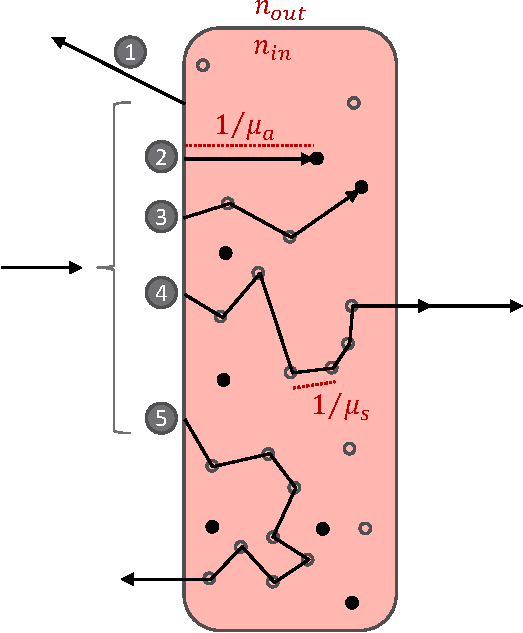
\includegraphics[width=.35\textwidth]{fig/background/lightinteraction.pdf}
    \end{center}
    \caption{Possible interactions when light interfaces with tissue. The pink rectangle represents tissue. White circles are scatterers. Black dots are absorbers.  (1) Light reflects without entering the tissue. (2) Light immediately gets absorbed. (3) Light scatters multiple times before being absorbed. (4) Light scatters multiple times before exiting the tissue on the opposite side it entered. (5) Light scatters multiple times but exits on the side it entered. } 
    \label{fig:lightinteraction}
\end{figure} 

The index of refraction, $n$, is a unitless number that describes how fast light travels through material~\cite{Wang2009}. It is used to determine how much the path of light is bent upon transitioning from one material to the next.  This is governed by Snell’s Law of Refraction~\cite{Wang2009}, $n_1 \times sin\theta_1= n_2\times sin\theta_2$, which define the angle of incidence, $\theta_1$, and angle of refraction, $\theta_2$, based on two media with indices of refraction $n_1$ and $n_2$. Thus, from Snell’s Law, we can also determine the amount of light that is reflected when reaching an interface (Figure~\ref{fig:lightinteraction}). 

Once photons enter a turbid media, they move in all directions and may be scattered or absorbed (Figure~\ref{fig:lightinteraction}). Absorption depends on the component concentrations of tissue~\cite{Nunez2018}. In the visible to near-infrared wavelength range, the primary absorption components include water, hemoglobin, pigment, and lipid~\cite{Du2006, Pogue2006}. The absorption coefficient, $\mu_a$ [$cm^{-1}$], is defined such that, when a photon propagates over an infinitesimal distance $ds$, the probability of absorption is $\mu_a\times ds$~\cite{Welch2010}. The absorption coefficient depends on the molar extinction coefficient of a given chromophore $\epsilon$ [$cm^{-1}\times M^{-1}$], and its Molar concentration, $c$. Thus, the absorption coefficient per wavelength is 

\begin{equation}
    \mu_a(\lambda) = log(10) \sum_{i=1}^{t}\epsilon_i(\lambda)\times c_i~\cite{Nunez2018}. 
\end{equation}
where t is the total number of absorbing components in the tissue. From this, we deduce that $1/\mu_a$ is the average path length traveled by a photon before being absorbed. 

Light entering a tissue can also undergo scattering events, events during which directionality changes occur due to biological structures within the media (Figure~\ref{fig:lightinteraction}). In the visible to infrared wavelength range, the primary scattering components in biological tissue are protein, fat, and mitochondria~\cite{Du2006, Pogue2006}. Analogously, the scattering coefficient, $\mu_s$, is defined such that, when a photon propagates over an infinitesimal distance $ds$, the probability of scattering is $\mu_s\times ds$~\cite{Welch2010}. Additionally, we model the probability distribution of scattered photons by an angular function known as the anisotropy factor, $g$~\cite{Wang2009}. Since $g$ is based on the scattering angle, the closer to 1.0 $g$ is, the more likely the photon is to be scattered in the forward direction. To account for this anisotropy factor, we define the reduced scattering coefficient, $\mu_s^{'}$, as 
$\mu_s^{'} = \mu_s(1-g)$~\cite{Wang2009}. The average distance traveled by a photon between scattering events is $1/\mu_s$.

\subsection{Components of Optical Measurement Systems}
Optical systems are composed of three elementary blocks: a source that radiates light, a sample through which light propagates, and a detector that measures the light intensity after photons have traveled through the sample~\cite{Webster2010}. Although there are numerous types of sources and detectors, here, we highlight only the types used in the optical systems developed for this thesis. 

\ac{LED} are devices that radiate light when a current passes through them~\cite{Webster2010}. They are ubiquitous in modern electronics due to being inexpensive and requiring minimal power to operate. In our \ac{MOXI} system, we leverage the white LEDs used for flash photography common in most smartphones. Our \ac{MOBI} system uses dual-wavelength \ac{LED}s chosen to optimize propagation within the brain layers. Arrays of \ac{LED}s are used in conjunction with digital micromirrors to project color images from projectors. Our \ac{OMCI} system uses an \ac{LED} projector to shine patterns to scan the surface of the breast. For certain applications, it is better to have a light source that does not spread out much. Lasers (Light Amplification by Stimulated Emission of Radiation) are light sources that produce very narrow beams of light. In \ac{OMCI}, we use a laser to input light into a projector to project patterns onto the breast. 

Detectors are devices used to measure light. Photodiodes are the reverse of \ac{LED}s---they convert light into electrical current~\cite{Webster2010}. Their cost tends to be relative to their sensitivity. \ac{MOXI} and \ac{MOBI} use inexpensive photodiodes chosen to be sensitive to the wavelengths of their associated \ac{LED}s. \ac{OMCI} uses cameras to detect the reflection and transmission of projected patterns. These cameras capture light through a small lens using a tiny array of microscopic detectors. 

The measured light, in combination with the known type of source, allows for the determination of biological structure, function, and molecular characteristics of the tissue through which the light propagated. For example, the detection of photons from particular wavelengths allows us to compute concentrations of oxygenated ($HbO_2$) and de-oxygenated ($HbR$) hemoglobin in tissue. From this, we can infer parameters such as total hemoglobin concentration and tissue oxygen saturation~\cite{Nunez2018}. 
%From this, we can infer parameters such as total hemoglobin concentration (THC=HbR+HbO_2) and tissue oxygen saturation (S〖tO〗_2=  (HbO_2)⁄((HbR+ HbO_2)))[3]. 

\subsection{Optical Phantom Fabrication}
Phantoms are objects with optical properties that mimic human tissues~\cite{Pogue2006}. They are common for evaluating the performance of \ac{NIR} imaging systems~\cite{Pogue2006}. To mimic \ac{NIR} light propagation due to components within biological tissue, phantoms typically attempt to mimic the reduced scattering coefficient ($\mu_s^{'}$) and the wavelength-dependent absorption coefficient ($\mu_a$) in biological tissue~\cite{Dempsey2017}. Traditionally, these phantoms are created using recipes that involve a mix of scattering agents and absorbing pigments with a base~\cite{Hebden1995,Dong2015}. The geometry of the phantom is typically created using either mold casting~\cite{Hahn2012,Mobashsher2014} or spin coating~\cite{Park2013}. While useful for simple phantoms, these methods fall short in supporting complex geometries needed for phantoms requiring structural and physiological properties, such as when DOT is used to image the brain~\cite{Hebden2002,Villringer1997}. Thus, a new method to manufacture phantoms with spatially varying optical properties and anatomically accurate geometries is needed to support the system development, calibration, and testing of new imaging protocols~\cite{Cerussi2012,Diep2015}.  


%%% Section
\section{Imaging Modalities}
\label{chap:background:modalities}
\subsection{Pulse Oximetry}
\subsection{Functional Near-Infrared Spectroscopy}
\subsection{Diffuse Optical Tomography}
\subsection{Structured-Light Imaging}



%%% Section
\section{``-ilities'' of Near-infrared Imaging Systems}
\label{chap:background:ilities}



%%% Section
\section{Thesis Aims}
\label{chap:background:aims}


% --- EOF ---
% moxi.tex:

\chapter{MOBILE-PHONE-BASED OXIMETER (MOXI)} % all caps please
\label{chap:moxi}
This is where the writing goes. 


\section{Introduction} %significan
\label{chap:moxi:introduction}



\section{Methods}
\label{chap:moxi:methods}



\section{Results}
\label{chap:moxi:results}



\section{Discussion}
\label{chap:moxi:discussion}




% --- EOF ---
% moca.tex:

\chapter{MODULAR OPTODE CONFIGURATION ANALYZER (MOCA)} % all caps please
\label{chap:moca}

%%% Section %%% 
\section{Introduction}
\label{sec:introduction}
Functional near-infrared spectroscopy (fNIRS) is an emerging neuroimaging technique to non-invasively measure brain activity using non-ionizing light~\cite{Ferrari2012}. Unlike functional magnetic resonance imaging (fMRI)~\cite{Heinzel2013} that requires high-strength magnetic fields and large scanners, fNIRS utilizes near-infrared (NIR) light to detect brain activation by measuring the associated hemodynamics. The portability of fNIRS positions it as a competitive imaging modality to address some of the challenges of conventional neuroimaging techniques, such as fMRI and magnetoencephalography (MEG), including a lack of wearability for continuous monitoring, limited temporal resolution, and need for subject immobility during use~\cite{Yucel2017}. It has shown great promise for safe and long-term monitoring of brain activity and is increasingly used in studies for behavioral~\cite{McDonald2018} and cognitive neurodevelopment~\cite{Aslin2015, Vanderwert2014, Wilcox2015, Soltanlou2018}, language~\cite{Quaresima2012, Rossi2012}, psychiatric conditions~\cite{Ehlis2014, Kumar2017}, stroke recovery~\cite{Yang2019}, and brain-computer interfaces~\cite{Naseer2015, Ahn2017, Hong2018}. 

Despite an exponential growth in the number of applications~\cite{Boas2014, Quaresima2019} and publications~\cite{Yucel2017} in recent years, many fNIRS systems still employ fiber-based, cart-sized instrumentation~\cite{Scholkmann2014} that place limits on both channel density and the use of fNIRS in natural environments. Although fiber-based high-density~\cite{Eggebrecht2014} and portable~\cite{Wheelock2019} fNIRS systems have been demonstrated, the use of fragile fiber optics cables, stationary external source/detector units~\cite{Oxymon2017, Techen2018}, and the need for individual and specialized headgear for specific tasks have motivated the fNIRS community to investigate more flexible modular and fiber-less designs~\cite{Zhao2017, Curtin2018}.

The modular fNIRS architecture is based on utilizing elementary optical source and detector circuits (modules) as repeating building blocks to form a re-configurable probe~\cite{Zhao2017}. This modular architecture offers significantly improved portability, scalability, flexibility in coverage, and fabrication cost~\cite{Zhao2017}. By avoiding the use of fragile optical fibers, modular fNIRS systems permit the use of light guides to directly couple light sources and detectors to the scalp, significantly reducing signal loss due to fiber coupling. The lightweight and compact modules also make wearable fNIRS and continuous monitoring in mobile environments possible~\cite{Yucel2017, Park2018}. In addition, the ability to use both intra-module (within a single module) and inter-module (source and detector on different modules) channels allows for high density probes with varying source-to-detector separations (SDS) that increase measurement density and tissue depth sampling, resulting in enhanced signal quality, and easy removal of physiological noise~\cite{Gregg2010}. 

Despite these perceived benefits, the task of designing a modular fNIRS probe can quickly grow in complexity as the number of modules increases. While parameters can be empirically determined when designing a single module, understanding the trade-offs among a large array of parameters, including module shape, module size, optode quantities, and optode locations, and each parameter's effects on the final probe can become a daunting task. Not only do most published modular fNIRS studies largely focused on the design of a single module without addressing the effect of these module- and probe-level parameters on the final probe, the current literature also does not provide a means to compare probes composed of different module designs.

Aside from the challenges of determining these modular probe core parameters, other factors such as mechanical, ergonomic, safety, usability, optoelectronic, and data communication considerations~\cite{Zhao2017} also play important roles in achieving the desired performance. For example, mechanical features such as optical coupling and electronic circuitry encapsulation must be considered alongside ergonomic considerations such as comfort, weight, and robustness. Additionally, the use of high density light sources in such modular probes brings about additional safety considerations, such as heat dissipation, driving voltage, and battery life. Moreover, optoelectronic considerations arise from the use of specialized optodes with narrow emission bandwidths, high gains, low noise, and fNIRS-optimized wavelengths. Not only are these specialized optodes more expensive due to their niche applications and characteristics, they also require more complex control electronics for driving optodes and acquiring data. With such dense coverage, complex encoding strategies such as frequency~\cite{Maki1995} multiplexing become a necessity for obtaining high density data acquisition to achieve sufficient spatial and temporal resolution. Finally, while previously reported modular fNIRS systems often employ daisy-chain communication protocols to connect multiple modules on a single bus~\cite{Chitnis2016, Bci2017, Zimmermann2013, Funane2017, Zhao2019}, the design of physical inter-module connections~\cite{Zhao2021}, the synchronization method between modules~\cite{Zhao2017}, and the transfer of acquired data become increasingly complex with high module counts and branching connections.

Along these lines, a number of fNIRS data analysis packages exists~\cite{Huppert2009, Santosa2018, Hernandez2020}. However, they focus on the statistical analysis of the data ~\cite{Hernandez2020,Huppert2009, Santosa2018} to enhance its quality and provide guidance on post-processing steps such as motion artifact correction~\cite{Huppert2009}. While some other tools exist to assist in the probe design~\cite{Brigadoi2018, Machado2018, ZimeoMorais2018, Aasted2015}, most of these tools are designed to work in a highly constrained design space, where the probe parameters are mostly pre-determined by the user. As a result, the best practices and trade-offs in modular probe design such as tessellation, connection, or re-orientation are poorly explored and understood. Therefore, the community is in great need of an easy-to-use software tool to assist the exploration of and quantitative comparisons among countless parameter choices in a modular probe design and to perform a limited degree of optimization within a well-constrained configuration. 

A fully-automated probe design and optimization pipeline is impractical without application-dependent design constraints. Instead, we report a simplified, easy-to-use software toolbox to help designers navigate the vast parameter space of a modular probe. We also share a number of fundamental modular probe design strategies, discovered through our explorations via this toolbox, that are not widely recognized or previously studied. The entire workflow has been implemented into an open-source, MATLAB-based toolbox called Modular Optode Configuration Analyzer (MOCA~\cite{Vanegas2020}). MOCA supports a list of commonly used module shapes, user-defined optode layouts, and region-of-interest (ROI) coverage, and can produce quantitative performance metrics such as distributions of source-detector (SD) separations, sensitivity maps, and spatial multiplexing groupings. These performance metrics also allow comparisons between different designs of modular probes. Although MOCA is not designed as a fully-automated software that produces ``optimal'' probes regardless of application, its unique capability to describe and sweep modular probe parameters in operator-guided interrogations offers valuable perspective to start approaching the complex modular hardware design problem and make informed comparisons between well-constrained design choices.

The remainder of the paper is outlined below. In Section~\ref{sec:overview}, we discuss the relevant design considerations when developing a modular probe using MOCA. We specifically focus on the parameterization of the modules, processes required to assemble modules into functional probes, and related performance metrics for system characterization and comparisons. In Section~\ref{sec:results}, we demonstrate MOCA's capability in designing full-head probes using a variety of module shapes and compare their trade-offs regarding channel density, SD separations, and average brain sensitivities. Furthermore, we utilize MOCA to showcase potential improvements to published fNIRS probes by altering module orientations, spacing, and staggering layouts. In Section~\ref{sec:discussion}, we highlight a number of generalizable design strategies that were discovered via our experiments using MOCA, including the importance of considering module orientations, tiling strategies, and module spacing tuning, among others.


% mobi.tex:

\chapter{MODULAR OPTICAL BRAIN IMAGER (MOBI)} % all caps please
\label{chap:mobi}
This is where the writing goes. 



\section{Introduction} %significan
\label{chap:mobi:introduction}



\section{Methods}
\label{chap:mobi:methods}



\section{Results}
\label{chap:mobi:results}



\section{Discussion}
\label{chap:mobi:discussion}

% --- EOF ---
% omci.tex:

\chapter{OPTICAL MAMMOGRAPHY CO-IMAGER (OMCI)} % all caps please
\label{chap:omci}
\ac{OMCI} is a high-density breast multi-subsystem devide designed to be used in conjunction with existing x-ray mammography systems or as a standalone system for \ac{DOT}. It integrates four subsystems: a mechanical breast compression stage to resemble clinical mammography, a frequency-domain subsystem for recovering absolute tissue optical properties, a wide-field transmission-based diffuse optical subsystem, and high-resolution breast surface acquisition system. Although \ac{OMCI} is composed of four separate subsystems working in tandem, in this chapter, we will briefly provide an overall instrument description but will focus on design and characterization of the dual-camera structured light imaging (\ac{SLI}) breast shape acquisition system used for improving diffuse optical tomography image reconstructions.


\section{Introduction} %significance
\label{chap:omci:introduction}
Breast cancer is the most commonly diagnosed cancer in women worldwide with an estimated 1,918,030 new cases in 2022 in the United States alone~\cite{Siegel2022}. Screening and diagnostics of breast cancer is done through structural or functional breast imaging using multiple breast imaging modalities. X-ray mammography and \ac{DBT}) are the primary breast cancer screening techniques~\cite{Secretan2015} used for early detection to reduce mortality rates~\cite{Tabar2003}. Modalities such as magnetic resonance imaging (\ac{MRI}) and positron emission tomography (\ac{PET}) are used less frequently than x-ray due to their high cost and use of radioactive isotopes~\cite{Secretan2015}. Despite its recommendation for screening, not only does x-ray mammography expose patients to ionizing radiation but it also suffers from a high false-positive diagnostic rate~\cite{Tabar2003, Elmore1998}. The modality lacks both strong structural contrast between healthy and tumor tissue, and the ability to quantify tissue functions to assess benign versus malignancy~\cite{Leff2008}. These limitations have led researchers to investigate using \ac{DOT}) techniques to characterize the breast tumor's physiology to lower false-positive diagnoses. 

Unlike x-ray mammography, \ac{DOT} is an imaging modality that uses non-ionizing \ac{NIR} radiation to yield three-dimensional (3-D) maps of the optical properties of illuminated tissue~\cite{Boas2001, Dehghani2009, Yamada2014, Hoshi2016}. Biological tissues' primary absorbers in the spectral window from around 600 to 1000~nm have relatively low absorption, allowing \ac{NIR} light to penetrate through centimeters of tissues~\cite{Gibson2005}. This allows the quantification of physiological properties such as hemoglobin concentration, blood volume, and blood oxygen saturation~\cite{Leff2008, Boas2001}. Malignant tumors generally demand a greater blood supply than their surrounding tissues, leading to increased light absorption that can be delineated using spectroscopy and imaging methods, making \ac{DOT} particularly useful for breast cancer imaging diagnosis~\cite{Wang2022, Vavadi2014, Flexman2013, Choe2009, Taroni2005}. Unfortunately, \ac{DOT} images are known for low spatial resolution largely caused by the high scattering properties of biological tissues~\cite{Boas2001}. 

The low spatial resolution of \ac{DOT}~\cite{Li2010} can be improved by a multi-modal approach with x-ray mammography~\cite{Zimmermann2017, Deng2015, Deng2015a, Fang2009a}. The high scattering present in the breast tissue redirects photons to traverse large overlapping probing volumes before their detection, greatly reducing the locality of the measurements and resulting in blurry images. Mathematically, this is reflected as the severe ill-posedness of the inverse problem. Parallel-plate compression of breast tissues has been used in an x-ray mammography scan to minimize overlapping tissues and has also been explored for a number of standalone~\cite{Choe2009, Culver2003} and multi-modal \ac{DOT} breast imaging systems~\cite{ZhuReview2020, Fang2009a, Krishnaswamy2012}. Multi-modal imaging approaches have been developed by leveraging tissue structural priors obtained from high-resolution imaging methods such as magnetic resonance imaging~\cite{Ghussein2013,Ntziachristos2002} and ultrasound~\cite{Zhu2010}. These approach leverage the advantages of multiple modalities---they leverage high quality structural images to constrain the \ac{DOT} inverse problem for more accurate tissue physiology reconstructions. 

Additionally, the \ac{DOT} reconstruction can also be improved by constraining the inverse problem through more accurate surface representations of the breast. Obtaining breast surface information to aid quantitative analysis of imaging data has garnered interest from a number of applications, including \ac{DBT}~\cite{Rodriguez2017} and \ac{MRI} scans~\cite{Pallone2014, Ortiz2012}. For multi-modal \ac{DOT} systems, the 3-D shape of the breast can be estimated using the structural imaging modality such as \ac{DBT}~\cite{Fang2011} or \ac{MRI}~\cite{Brooksby2006}. When a 3-D imaging modality is not available, two-dimensional (2-D) mammography~\cite{Deng2015a} has also been used to provide the shape information. In such case, a simple way to recover a 3-D breast surface is to extrude the 2-D breast contour along the compression axis~\cite{Kruger2013, Kalbhen1999}, or sweep the 2-D breast contour along the contour line extracted from an orthogonal view~\cite{Kita1998}. These methods either rely on assumptions about the 3-D location of certain features (e.g. mamilla position) or assume a constant curvature of the breast along the sweeping direction. For more accurate reconstructions of tissue optical properties, especially near the surface, measuring 3-D breast surface accurately can be greatly beneficial.

Accurately acquiring breast 3-D surface shapes has gained clinical acceptance due in large part to the plastic and reconstructive surgery communities~\cite{Chang2015, Losken2005}. The two prominent techniques for 3-D breast surface imaging are stereophotogrammetry and laser scanning~\cite{Yang2015}. Stereophotogrammetry works by overlaying multiple images of an object taken from different view angles and triangulating the location of the object based on matching features in the multiple images~\cite{Ju2016, Galdino2002, FangOSA2012}. In addition to requiring multiple cameras to increase accuracy~\cite{Henseler2012}, this technique is also heavily influenced by lighting conditions since features need to be extracted from multiple viewpoints~\cite{Henseler2011}. Another limitation is the ``ptosis error'' seen during scanning of ptotic or larger breasts~\cite{Nahabedian2003}. This arises due to the small field of view of stereophotogrammetry systems, leading to inaccuracies in breast surface and volume estimations due to the portions of the breast that are not illuminated. Laser scanning is a surface imaging technique in which rays from a laser beam are reflected off an object and detected by a detector~\cite{Kovacs2006}. Although laser-based acquisition systems can produce more accurate surfaces~\cite{Kovacs2006b}, these systems tend to be expensive~\cite{Kovacs2007, Koch2011} and require the need for very precise setups~\cite{Thomson2009}. Recently, the use of patterned-lasers and orientation-sensitive detectors has led to an increase in portable 3-D laser scanning devices~\cite{Kuzminsky2012}. While low-cost laser-based depth sensors have been widely deployed in game consoles such as Xbox or PlayStation, they are only designed to achieve relatively low spatial accuracy compared to dedicated 3-D scanners. Still, patterned-laser-based surface acquisition systems generally require a minimum scanner-to-target distance of 35~cm~\cite{Ametek2002, Artec3D2022}. Additionally, their typical housing is too large to fit between mammography compression plates~\cite{Artec3D2022, Pallone2014}. Bulky instrumentation and long minimum working distance requirements make stereophotogrammetry and laser scanning techniques infeasible in the confined, low-light mammography setting. 

Another widely used 3-D surface acquisition technique is \ac{SLI}~\cite{Yang2020, Zhang2018}. \ac{SLI} works by illuminating an object with two-dimensional spatially varying patterns with a projector and capturing images from the illuminated object using cameras~\cite{Geng2011}. The distortion of the specially designed patterns provides information regarding the shape of the object. Calibration of the camera-projector system is easily done by capturing images of a known planar pattern (e.g. a checkerboard). With the ability to use off-the-shelf components, a simple setup with a single projector and camera, and a robust and simple calibration method, \ac{SLI} is positioned to provide accurate, fast, and cost-effective breast surface scanning~\cite{Yang2020}. However, similar to most patterned-laser surface scanners, commercially available \ac{SLI} systems have long minimal working distance requirements and large assemblies that cannot readily fit within the confined mammography compression plates~\cite{Zhang2018, Rodriguez2017}.

Our approach to lowering false-positive diagnoses is two-fold. We first aim to improve \ac{DOT} reconstruction through more accurate surface representations of the compressed breast. Second, we aim to develop a standalone \ac{DOT} breast imaging system that leverages structural information through the registration of the \ac{DOT} reconstruction with prior x-ray mammographies. Our group has primarily focused on the latter through the development of both multi-modal \ac{DOT} reconstruction algorithms~\cite{Deng2015} and multi-modal (\ac{DOT} and \ac{DBT}) instrumentation that can work independently~\cite{Carp2006,Carp2008,Carp2013} or in conjunction with existing mammography systems~\cite{Fang2009,Zimmermann2017}. The approach to build \ac{DOT} systems that can work independently and integrate with existing mammography systems is commercially intriguing, since it can lower acquisition costs and maximize previous investments made into clinical instrumentation. We will take this same approach in our first aim---that is, the \ac{SLI} surface acquisition system we build will also have the capability to function independently or be easily integrated into existing mammography systems. 

In this chapter, we first describe the overall \ac{OMCI} instrument and its subsystems. We then describe the design of the \ac{SLI} breast scanner and detail the methods for adaptive illumination for subject-specific skin tones as well as approaches to reduce specular reflection from the compression plates. Next, we compare several traditional surface acquisition methods that leverage mammography images against our \ac{SLI}-based breast surface acquisition system and quantify the impact of improved breast surface acquisition on the recovery of breast lesions using a series of simulations. Finally, we demonstrate \ac{OMCI}'s use on healthy volunteers.



\section{Methods}
\label{chap:omci:methods}

%%% Subsection %%%
\subsection{OMCI Instrument}
\begin{figure}[]
    \begin{center}
    \subfigure[]{\label{fig:OMCISystemA}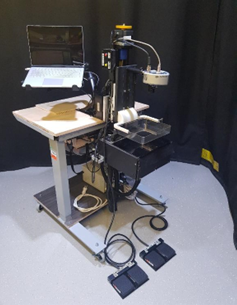
\includegraphics[width=.4\textwidth]{fig/omci/OMCISystemImage_1.png}}
    %\subfigure[]{\label{fig:OMCISystemB}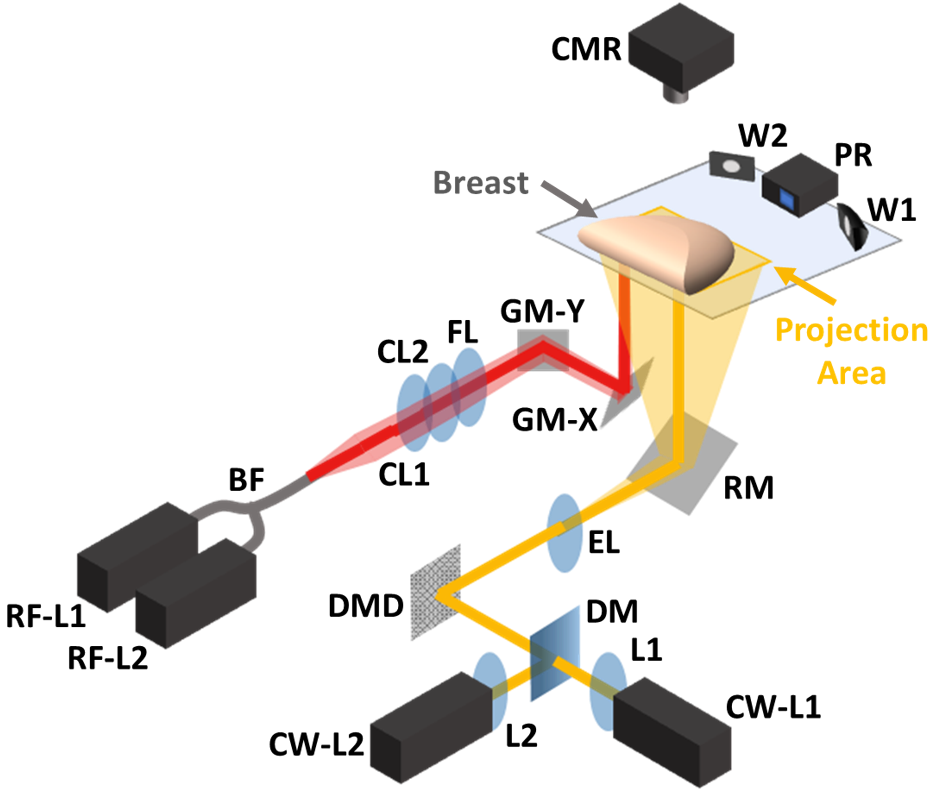
\includegraphics[width=.5\textwidth]{fig/omci/OMCISystemSketch.png}}
    \end{center}
    \caption{The \ac{OMCI} system in its fully compressed state. } 
    \label{fig:OMCISystem}
\end{figure} 

%\subsubsection{Mechanical stage and auxiliary sensors suite}
\ac{OMCI} is composed of a linear stage mounted on a vertical rotary stage. The breast is compressed by a pair of acrylic plates, with one plate mounted at the stationary end of a linear stage (MN10-0160-M02-31 BiSlide, Velmex, NY, USA). Under the bottom compression plate is a box that encloses many of the optical components of \ac{OMCI}. An acrylic mammography compression plate is mounted on the moving gantry of the linear stage, allowing for a plate separation ranging from 300~mm (fully released) to 0~mm (fully closed). A linear encoder (ETI Systems, Carlsbad, CA, USA) is connected between the pair of compression plates to measure their separation. The entire breast compression assembly is mounted on a rotatory table (306045-1-s-M04-C376, Lintech, Monrovia, CA, USA), controlled by a foot pedal to permit mammography-like lateral-oblique compression. A motor driver interface (VXM-2, Velmex Inc., USA) allows both stages to be actuated independenly by their stepper motor (NEMA 34 PK296 Stepper Motor, Oriental Motor Corporation, MA, USA). Two limit switches (BiSlide Push Button, Velmex Inc., NY, USA) confine the translation stage range. A reed switch (L06 Non-Contact Reed Switch, LinTech Motors, CA, USA) is used for homing the rotary stage. Four load sensors (SEN-10245, SparkFun, CO, USA) hold up the bottom compression plate and measure the pressure applied on the breast.  This design specifically enables registration of structural information from separately acquired mammography scans with the \ac{DOT} images using the methods detailed in our previous studies~\cite{Deng2015}.

%\subsubsection{Galvo-based frequency-domain subsystem}
%\label{sec:RF}
While the breast is in compression, it is illuminated with an \ac{FD} and a \ac{WF} subsystem. Bulk tissue properties are determined using a \ac{FD} subsystem~\cite{Zimmermann2016} that utilizes two laser modules (HL6750MG and HL8338MG, Thorlabs GmbH, Germany) coupled to bifurcated fiber bundle (BFY400LS02, Thorlabs GmbH, Germany). The frequency multiplexed light is driven into the \ac{OMCI} box where a dual-axis galvo motor (GVS002, Thorlabs GmbH, Germany) redirects it onto different positions on the bottom of the compressed breast. A fixed detector on the top compression plate directs the light to a frequency-domain detector (C5331-04, Hamamatsu, Japan) for collection. The \ac{WF} subsystem illuminates the breast from below using a \ac{CW} projector (P300 Neo, Aaxa Technologies, USA) while a \ac{EMCCD} camera (Andor Luca R, Oxford Instruments, U.K) located above the compression plate samples the dual-wavelength light transmitted through the breast. Both the \ac{FD} and \ac{WF} subsystems are controlled through the \ac{OMCI} \ac{GUI} written in MATLAB. 


%%% Subsection %%%
\subsection{Dual-camera SLI breast surface scanning system}
\label{sec:sli}
\begin{figure}
	\begin{center}
	\subfigure[]{\label{fig:mammography_top}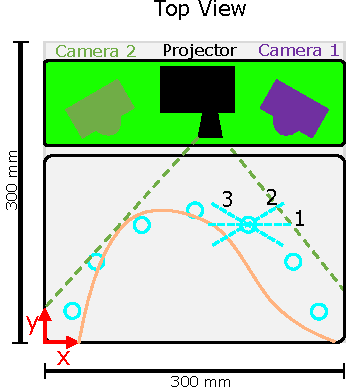
\includegraphics[height=5cm]{fig/omci/mammography_top.pdf}}
	\subfigure[]{\label{fig:mammography_side}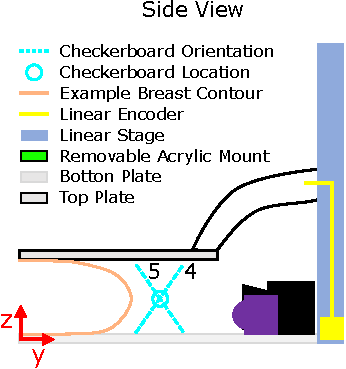
\includegraphics[height=5cm]{fig/omci/mammography_side.pdf}}
	\subfigure[]{\label{fig:mammography_setup}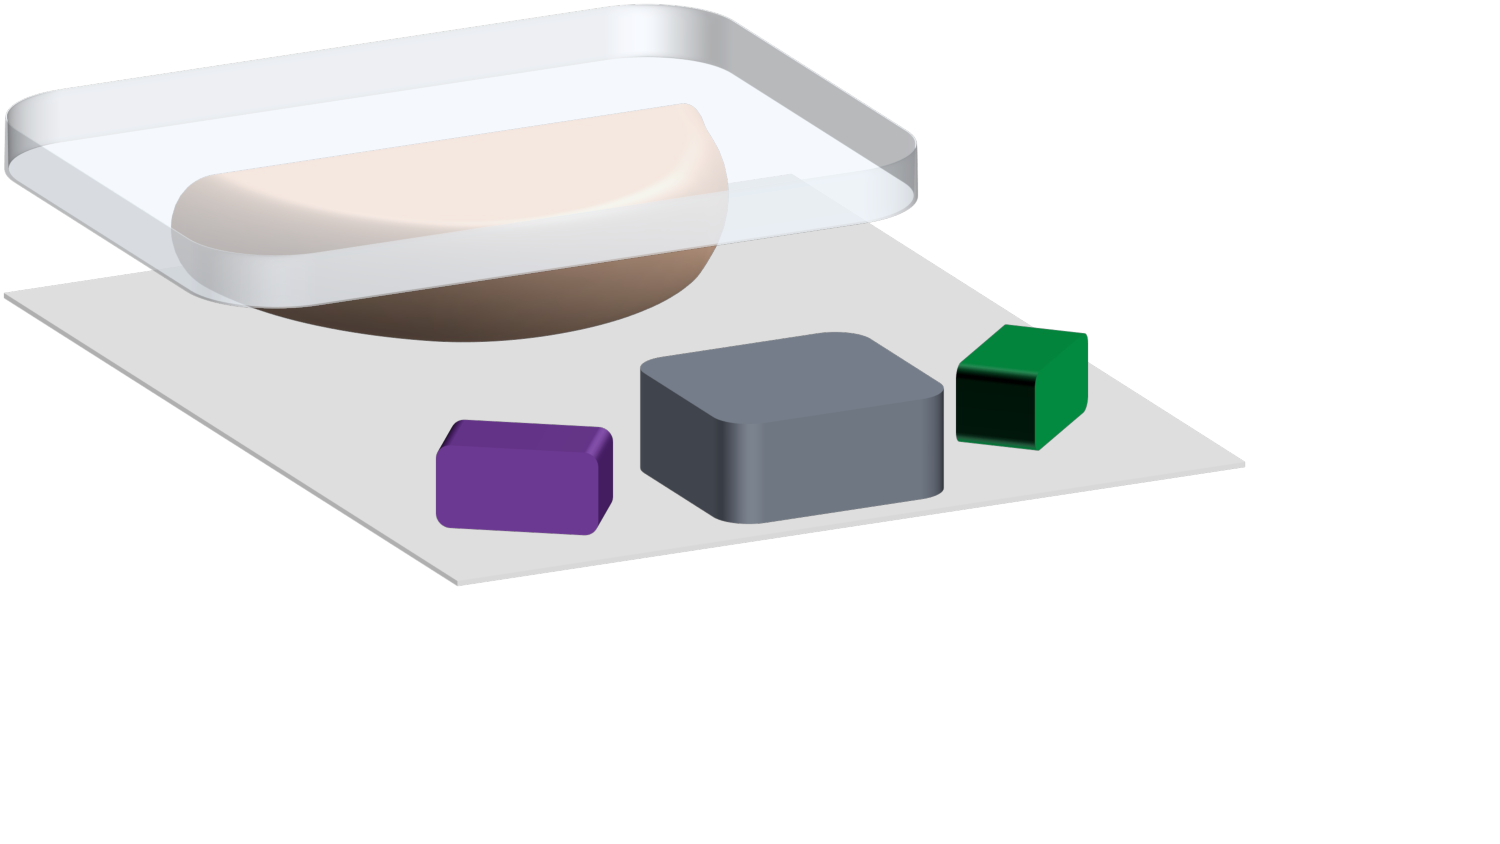
\includegraphics[width=5cm]{fig/omci/sli_model.pdf}}
	\end{center}
	\caption{ (a) Top-view of the breast compression compartment -- upper: \ac{SLI} system; bottom: horizontal cross-section (orange line) of the compressed breast with blue circles indicating the placement of the checkerboard used for system calibration. Numbers 1-5 indicate the 5 board orientations repeated at each location for calibration. (b) Side-view of the breast compression plates, showing the linear translation stage (blue bar on the right) and a linear encoder (in yellow), and  (c) 3-D rendering of the \ac{SLI} system, an acrylic bottom plate and an acrylic compression plate (top). } 
	\label{fig:mammographysetup}
\end{figure} 

The \ac{SLI} system is embedded between the compression plate to provide accurate measurement of the breast surface [Fig.~\ref{fig:mammography_setup}]. This low-profile \ac{SLI} scanner has a dimension of 30$\times$10$\times$4.8~cm$^3$ and is attached to the stationary compression plate, on the side facing the patient's breast [Fig.~\ref{fig:sli_setup}]. It consists of a central projector (P2-B DLP Pico Projector, AAXA Technologies, Irvine, CA, USA) and two USB cameras (C525, Logitech, Lausanne, Switzerland) to reconstruct a 3-D surface of the compressed breast. The \ac{SLI} scanner is designed to have a relatively short scanner-to-target distance, typically less than 15~cm, and a vertical profile of less than 3~cm to permit scanning breasts with a wide range of sizes. A laptop is used to control the data acquisition, including illumination pattern generation, projection, camera image acquisition, and translation stage control via an interface written in MATLAB (R2017b, Mathworks, Natick, MA, USA).

Gray-code-based binary patterns~\cite{Inokuchi1984} are sequentially illuminated onto the breast surface and captured using both USB cameras. These patterns are characterized by their pattern order, $P$. A pattern set of $P=3$ results in 3 sequences which are a reflected binary of the previous (``01'', ``0110'', and ``01100110''). Four bar patterns are created for each sequence (a horizontal black and white bar pattern, a vertical black and white bar pattern, and the complimentary pattern of each)~\cite{Sels2019}. The digits correspond to the white (``1'') and black (``0'') bars. In addition, a full-bright (white) and full-dark (black) pattern are added to each pattern set. Thus, a pattern set of $P=3$ results in $4\times P+2$ illumination bar patterns. Complimentary Gray-code-based illumination pattern sets are used due to their robustness to decoding errors~\cite{Moreno2012}. The two USB cameras have overlapping field-of-views and sequentially capture images of the breast during each illumination pattern at an exposure time of 250~ms. Dual-camera simultaneous acquisition allows the \ac{SLI} system to capture the curved surface of breasts of varied sizes without moving components. 

\subsubsection{Special data acquisition considerations}\label{sec:special}
% skin tone
Skin tone differences are known to affect light-based surface reconstruction accuracy, especially in low-light settings. To account for skin tone variations, the normalized illumination patterns are multiplied by a scaling factor $\alpha$ ranging from 0 to 1 to prevent camera saturation. The scaling factor for a camera is calculated prior to data acquisition by first illuminating a full-bright pattern with $\alpha=1$ onto the breast and capturing a single image using the camera. If the maximum pixel value of the captured image is above a preset threshold, $\alpha$ is decreased and the breast is re-illuminated with a full-bright pattern multiplied by the new $\alpha$ value. This procedure is repeated until the maximum pixel value of the captured image is less than 95\% of the camera's maximum allowable pixel value. This entire procedure takes an estimated 8 seconds to complete and is repeated for each camera.

\begin{figure}
	\begin{center}
	\subfigure[]{\label{fig:sli_setup}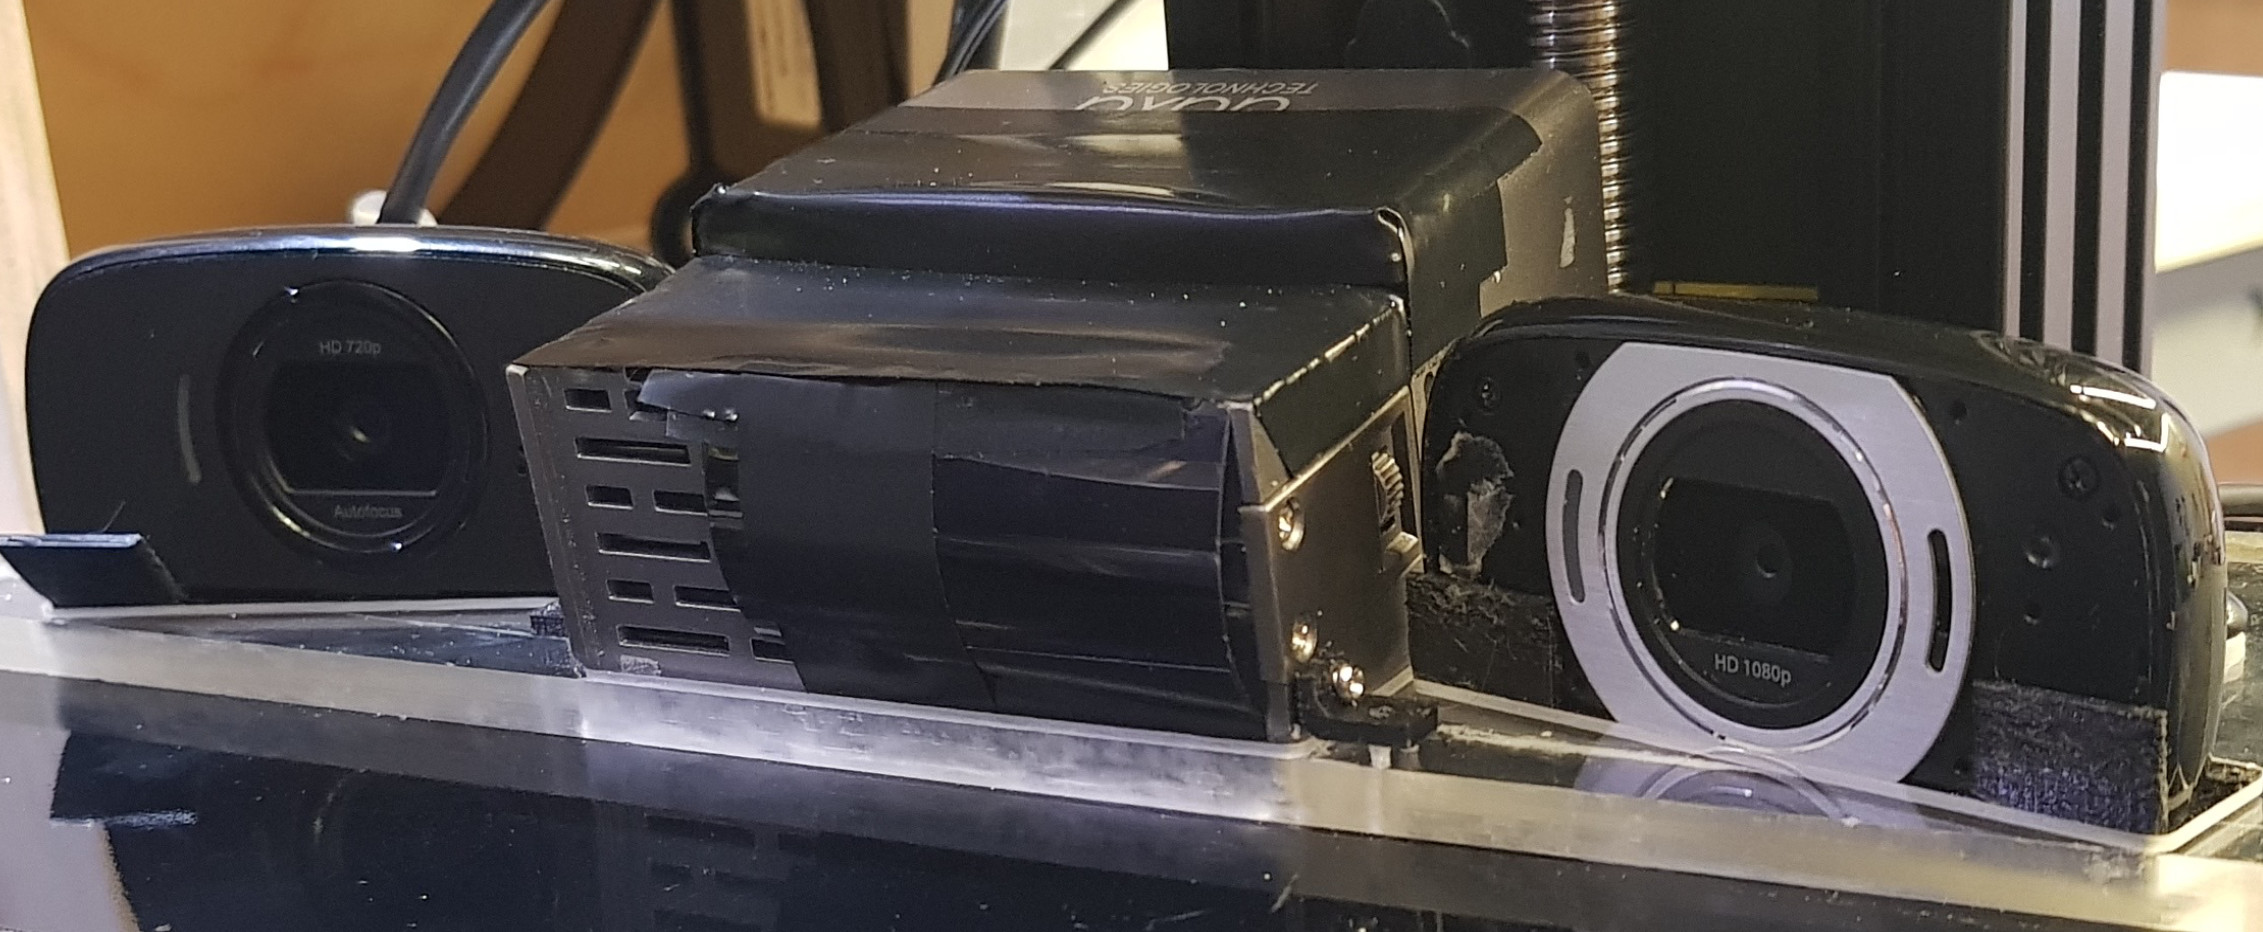
\includegraphics[height=2.4cm]{fig/omci/sli_photo.jpg}}
	\subfigure[]{\label{fig:artifact1}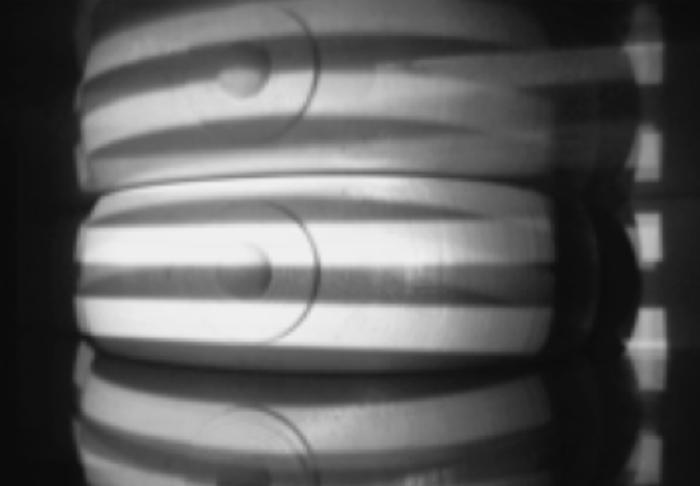
\includegraphics[height=2.4cm]{fig/omci/bars_artifact.png}}
	\subfigure[]{\label{fig:artifact2}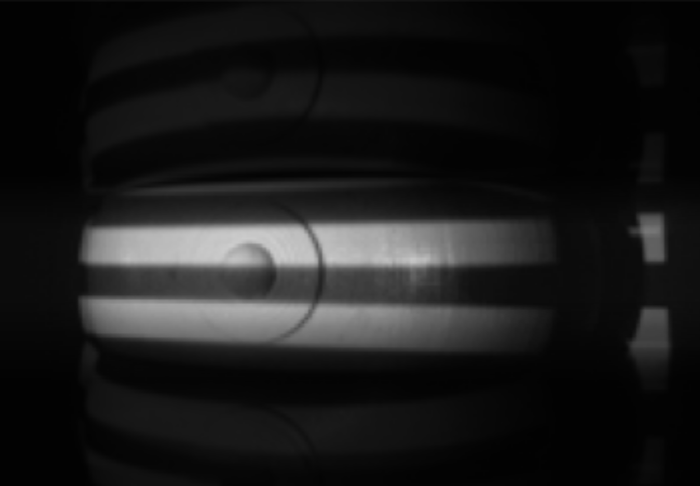
\includegraphics[height=2.4cm]{fig/omci/bars.png}}
	\end{center}
	\caption{(a) Front-view photo of the \ac{SLI} system. Cameras and projectors are embedded in an acrylic mount to prevent the need for re-calibration. (b) Horizontal bar patterns reflecting off the top compression plate and onto the breast show curved illumination bar artifacts when the scaling factor $\alpha$ is set to 1. In (c), we show the same illumination pattern with thickness-informed masking eliminating the curved bar artifacts by cropping the patterns exceeding the breast surface before projection. Additionally, the scaling factor is automatically calculated to prevent camera saturation.} 
	\label{fig:barartifacts}
\end{figure} 

% encoder-informed masking
Additionally, specular reflections from the acrylic compression plates, shown in Fig.~\ref{fig:artifact1}, can produce vertically mirrored breast surfaces. To minimize such specular reflection, we use dynamic pattern masking based on real-time separation readings provided by a linear encoder. By limiting the vertical span of the illumination patterns, the patterns are projected onto the compressed breast surface without generating strong direct specular reflections from the top and bottom compression plates, as shown in Fig.~\ref{fig:artifact2}.

\subsubsection{SLI system calibration and re-projection errors}
A standard \ac{SLI} camera-projector calibration is performed prior to image acquisition and is described in detail in~\cite{Moreno2012}. For each camera-projector pair, a checkerboard pattern is fully illuminated in multiple positions and the corner locations are estimated in the projector's default coordinate system using a robust pixel classification algorithm~\cite{Xu2007}. The camera and projector's intrinsic parameters (optical center and focal lengths) are estimated using a calibration method described in~\cite{Zhang2000} by fixing a world coordinate system to the calibration checkerboard plane. 

The projector's extrinsic parameters (rotation and translation from camera to projector) are calculated using a simple stereo camera calibration~\cite{Bouguet2004} that treats the projector as a secondary camera. This results in a rotation matrix and a translation vector relating the camera's coordinates to the projector's coordinates. Once the 3-D coordinates of all the corners of the checkerboard are computed using the camera's (and projector's) intrinsic and extrinsic parameters, the corners are ``reprojected'' onto all the images for which they appear. The re-projection error is defined as the average distance between the re-projected corner locations and the actual corner location. 

\subsubsection{SLI system acquisition}
The same acquisition procedures are used for both calibrating the system and acquiring breast shape measurements (Fig.~\ref{fig:sli_flowchart}). A single acquisition refers to the image capture of all illumination patterns by both cameras. Camera-projector calibration requires an acquisition at each checkerboard position. During breast measurements, the acquisition is preceded by the determination of the saturation scaling factor $\alpha$ and masking of the patterns. Patterns during calibration are not masked since the calibration is done with the system fully uncompressed. 

\begin{figure}
    \begin{center}
    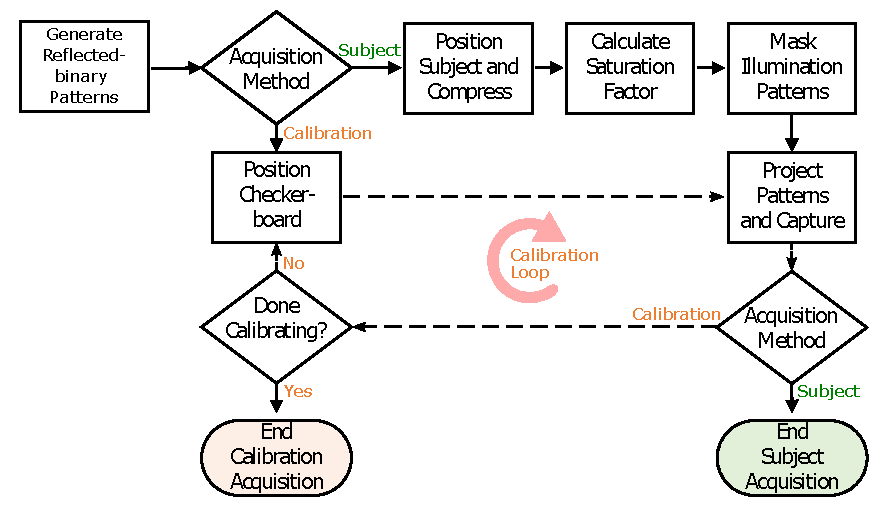
\includegraphics[width=.9\textwidth]{fig/omci/sli_flowchart.pdf}
    \end{center}
    \caption{Flow chart of image acquisition for both subject measurements and system calibration. Subject measurements calculate a saturation scaling factor and mask the illumination patterns prior to projecting patterns. System calibration measurements do not mask the illumination patterns and project at full intensity. The calibration loop (dashed lines) is repeated for each location and orientation of the calibration checkerboard.} 
    \label{fig:sli_flowchart}
\end{figure} 

%%% Subsection %%%
\subsection{Alternative breast surface reconstruction methods for assessing SLI surface accuracy}
To evaluate the accuracy of the \ac{SLI} system, we compare its output against alternative surface acquisition methods. Each method estimates the surface of a 3-D breast derived from a \ac{DBT} scan.

\begin{figure}
    \begin{center}
    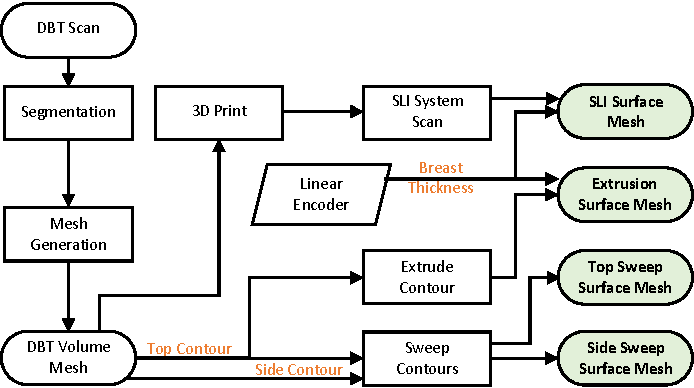
\includegraphics[width=.9\textwidth]{fig/omci/mesh_flowchart2.pdf}
    \end{center}
    \caption{Generation of breast surface meshes using multiple acquisition methods. The \ac{DBT} volumetric mesh is created from segmented scans. The extrusion surface mesh is created by extruding the top contour to the breast thickness. The top and side contours of the \ac{DBT} mesh are swept to create top and side surface meshes. The \ac{SLI} mesh is created by scanning a 3-D printed breast phantom and trimming the resulting point-cloud using the linear encoder measurements. The surface estimation error is calculated for each of the surface meshes by comparing the surface estimations to the \ac{DBT} mesh. All surface meshes are converted to volumetric meshes for validating the effect of surface estimation methods on inclusion reconstruction.}
    \label{fig:mesh_flowchart}
\end{figure} 

\subsubsection{Reference breast phantom fabrication}
Fig.~\ref{fig:mesh_flowchart} shows the process of creating surface meshes from \ac{DBT} scans. Scans were obtained from radiology data from \ac{TCGA} breast Invasive Carcinoma collection~\cite{Lingle2016}, available freely through The Cancer Imaging Archive~\cite{Clark2013}. The scan (ID: TCGA-AO-A03M) was chosen due to its large size and complex surface structure, allowing us to highlight the limitations of low field-of-view acquisition methods as well as traditional shape estimation methods that simply sweep a single breast contour. \ac{DICOM} slices were segmented into breast and non-breast regions using ITK-SNAP~\cite{Yushkevich2006}. Segmented slices were converted to a volumetric image and then into a 3-D mesh using a MATLAB toolbox Iso2Mesh~\cite{Fang2009} [Fig.~\ref{fig:mesh_dbt}].

\subsubsection{Single and double contour sweep-based surfaces}
Three alternative surface estimation methods are employed in addition to the \ac{SLI} surface acquisition method. These three methods use spline models of the \ac{DBT} breast contours from two different planes (Fig.~\ref{fig:mammographysetup}). The extrusion method creates a surface mesh by extruding the $x/y$ breast contour in the $z$ direction to the thickness of the \ac{DBT} breast measured by the linear encoder [Fig.~\ref{fig:mesh_extrude}]. The second and third methods utilize a curve-based sweep, in which a profile (shape) follows a path (contour) to create a 3-D model. In the ``top-sweep'' method, the $x/y$ breast contour profile is swept along the $y/z$ breast contour path [Fig.~\ref{fig:mesh_topsweep}]. Similarly, the ``side-sweep'' method uses the $y/z$ breast contour as the profile and the $x/y$ breast contour as the path [Fig.~\ref{fig:mesh_sidesweep}]. In both sweep methods, the profile normal is kept constant.

\begin{figure}
	\begin{center}
	\subfigure[]{\label{fig:mesh_dbt}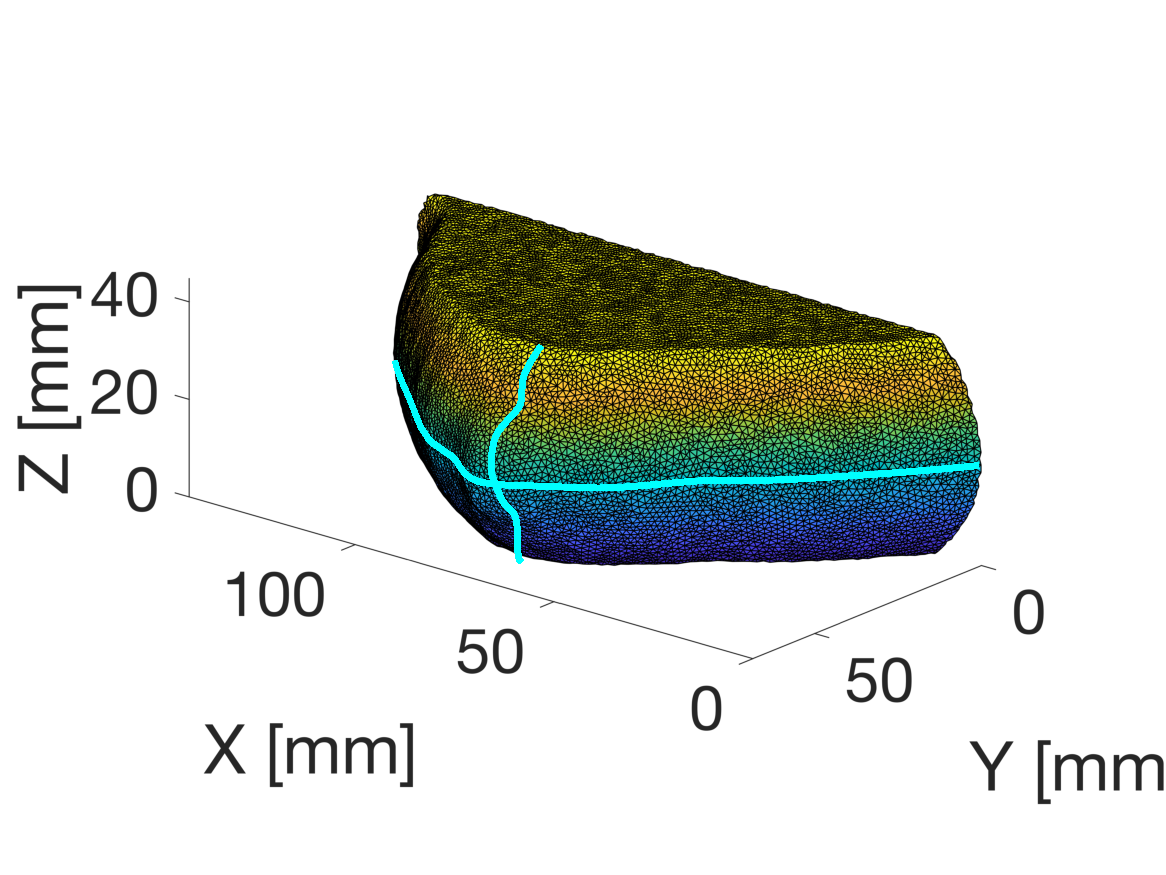
\includegraphics[width=.32\textwidth]{fig/omci/mesh_dbt.pdf}}
	\subfigure[]{\label{fig:mesh_extrude}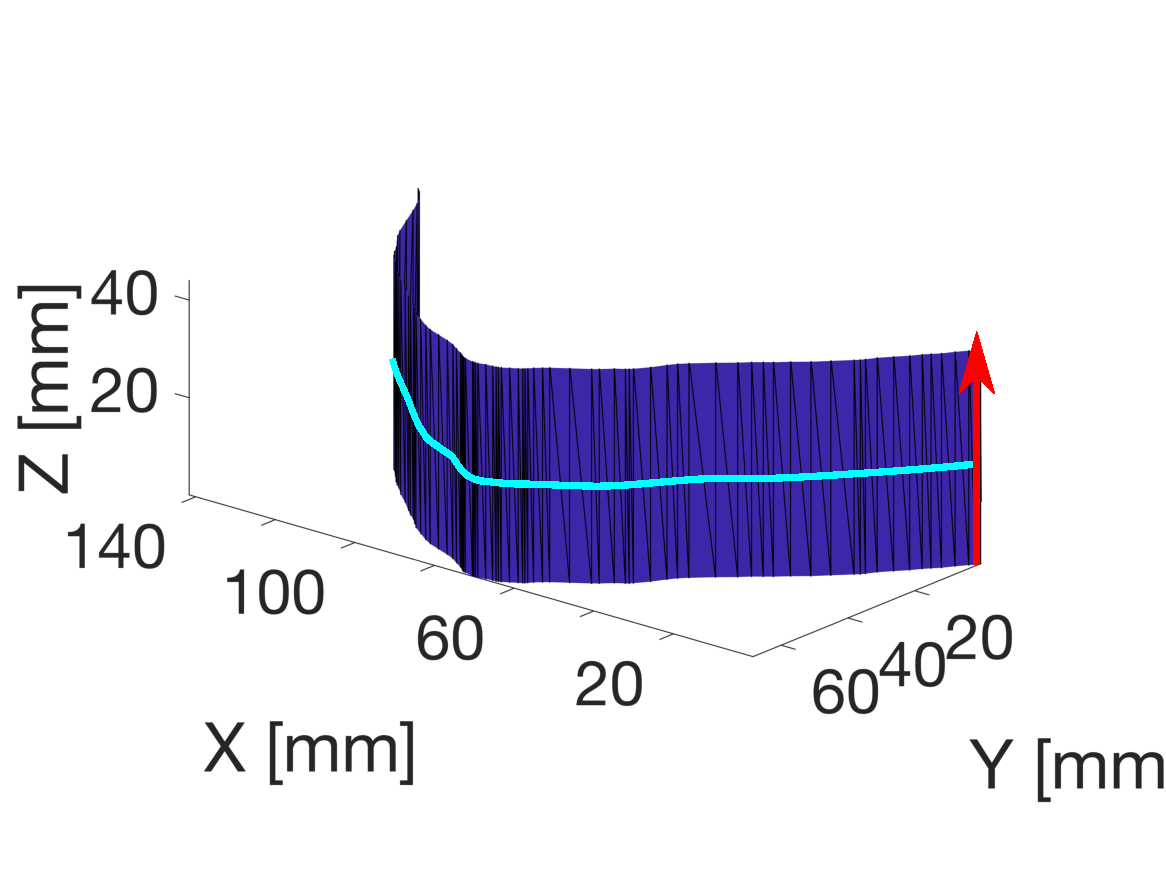
\includegraphics[width=.32\textwidth]{fig/omci/surf_ext.pdf}}
	\subfigure[]{\label{fig:mesh_topsweep}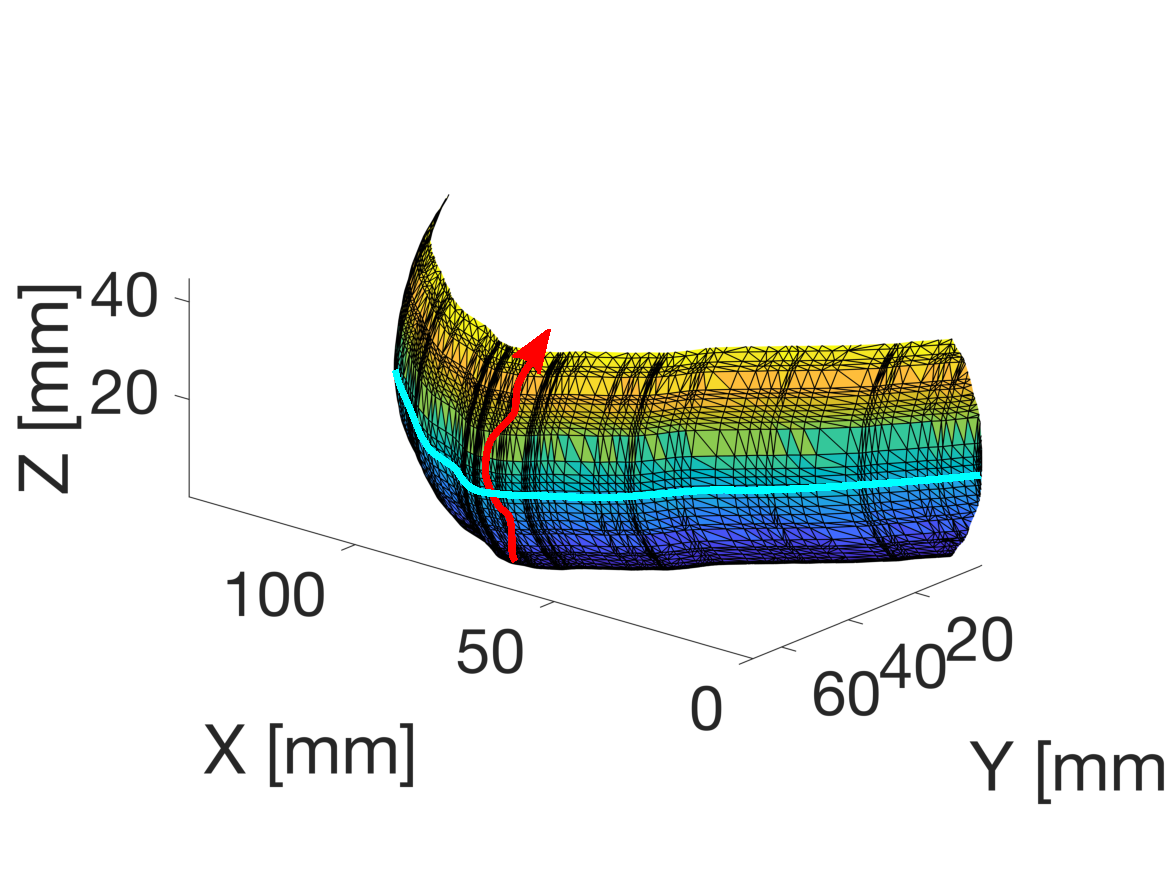
\includegraphics[width=.32\textwidth]{fig/omci/surf_top.pdf}}
	\subfigure[]{\label{fig:mesh_sidesweep}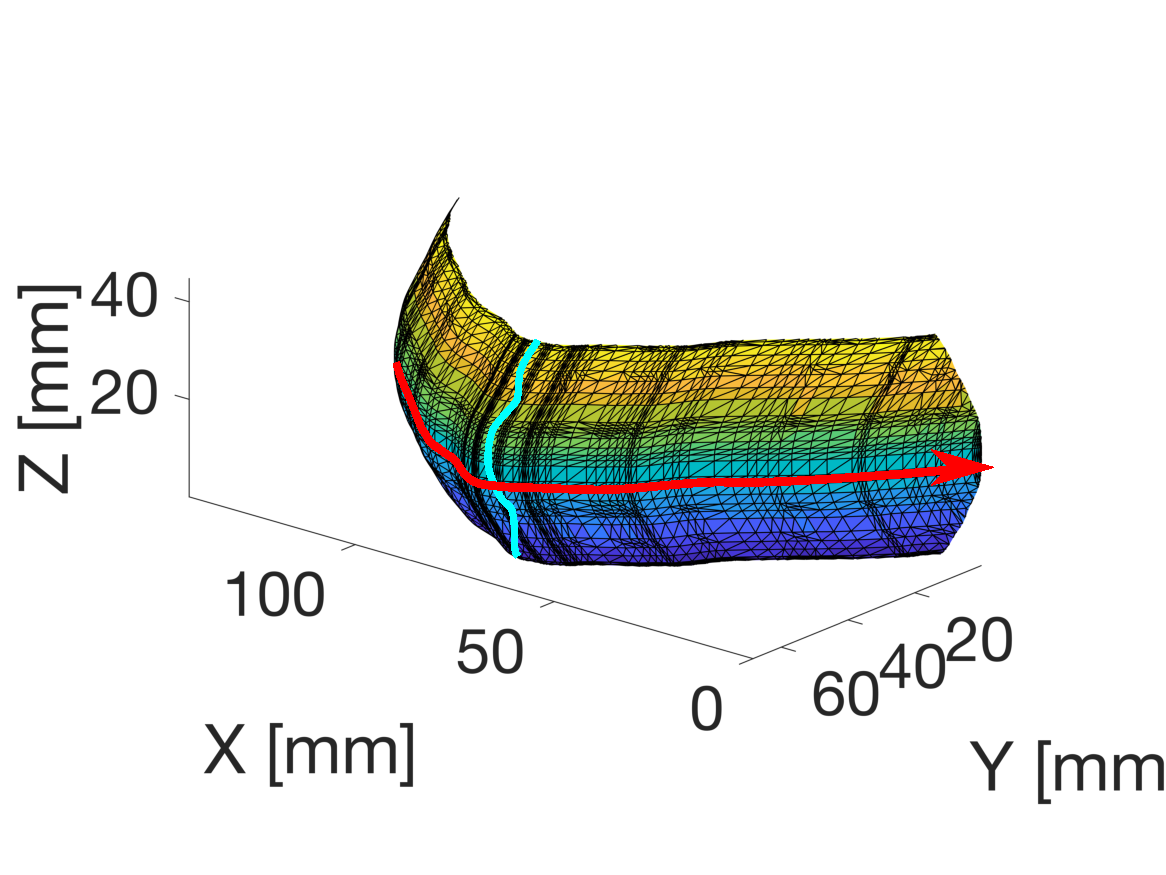
\includegraphics[width=.32\textwidth]{fig/omci/surf_side.pdf}}
	\subfigure[]{\label{fig:pcmergea}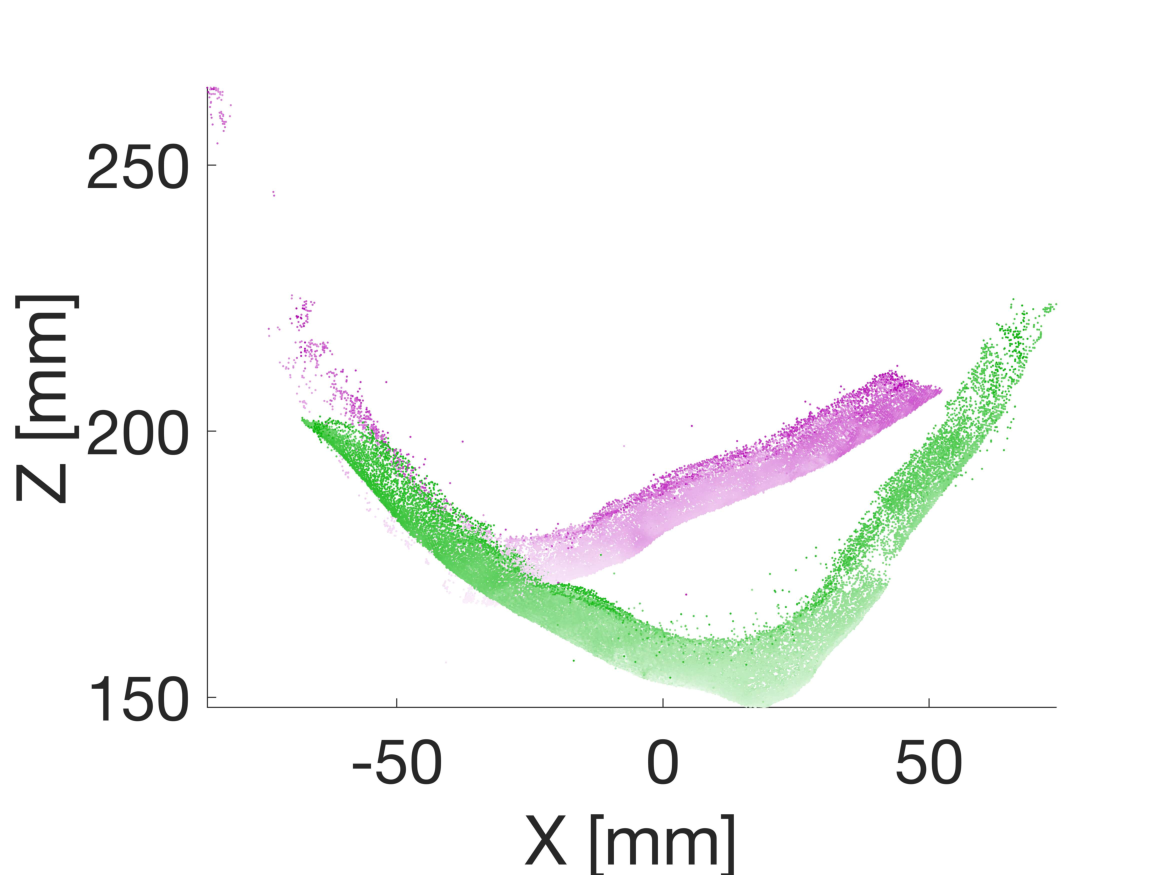
\includegraphics[width=0.32\textwidth]{fig/omci/PC_dual.pdf}}
	\subfigure[]{\label{fig:pcmergeb}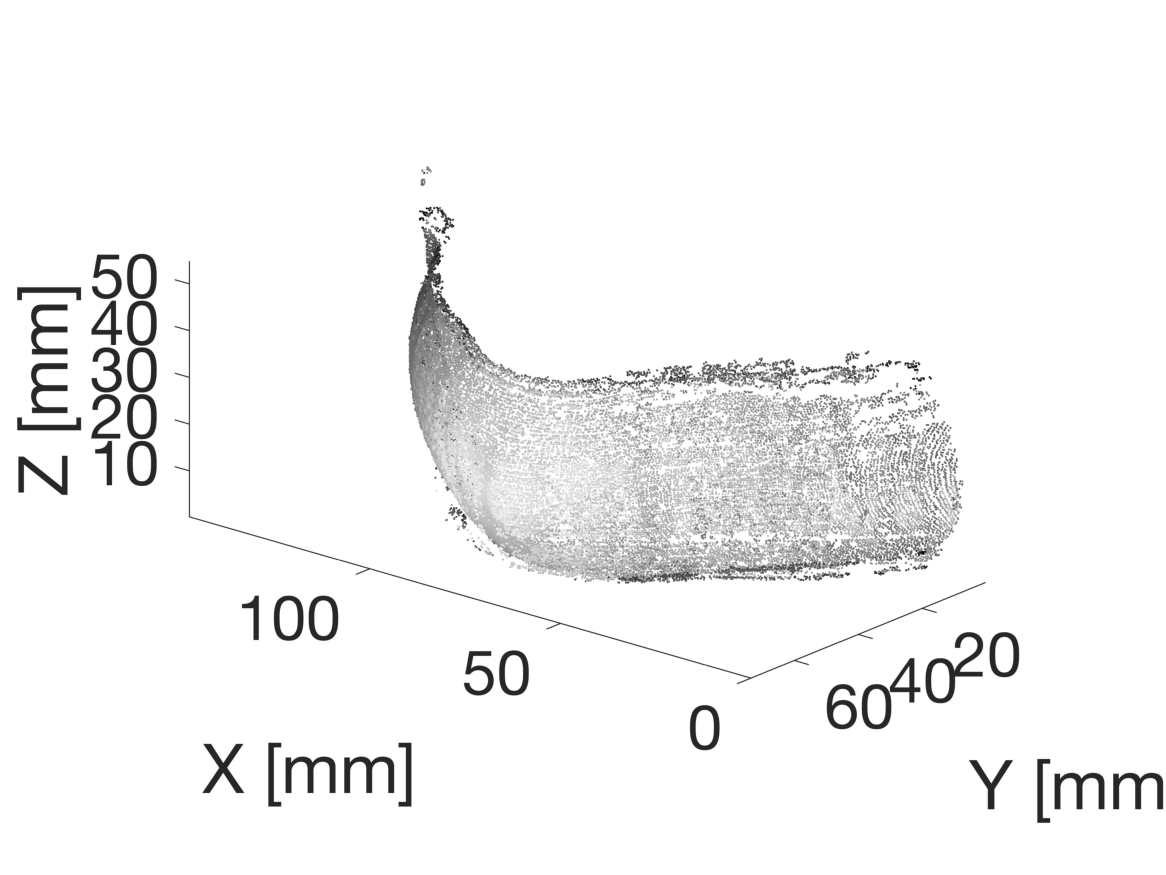
\includegraphics[width=0.32\textwidth]{fig/omci/PC_merged.pdf}}
	\end{center}
	\caption{(a) Surface mesh of a digital breast tomosynthesis model obtained from The Cancer Imaging Archive~\cite{Clark2013}. Blue cyan lines show the $x/y$ and $y/z$ breast contours from the top and side views. (b) Estimate of the \ac{DBT} surface using the extrusion method in which the contour (cyan) is extruded to the thickness of the breast along the $z$ axis. (c) The top-sweep method uses the $x/y$ contour as the profile (cyan) and the $y/z$ contour as the path to sweep (red). (d) The side-sweep method uses the $y/z$ contour as the profile (cyan) and the $x/y$ contour as the path to sweep (red). (e) point-clouds from both camera-projector pairs were generated by scanning a 3-D printed model of the \ac{DBT} breast using the \ac{SLI} system. The green (Camera 1) and magenta (Camera 2) point-clouds are in the respective camera coordinates. (f) Merged and denoised point-cloud in the projector's coordinates.} 
	\label{fig:meshes}
\end{figure} 

\subsubsection{Structured light imaging surface mesh generation}
The \ac{SLI} system estimates the surface of the compressed breast from the captured images while the breast is illuminated with Gray-code sequence patterns. Each camera-projector pair's extrinsic parameters are used to generate a point-cloud in each camera's reference frame using Scan3d-Capture~\cite{Moreno2012a} [Fig.~\ref{fig:pcmergea}]. The alignment of each camera-projector pair point-cloud is done by a rigid transformation of each point-cloud to the projector's coordinates. The point-clouds are then down-sampled using a box grid filter and merged to a single point with normal properties averaged~\cite{Pomerleau2013}. Denoising is then performed to remove outliers~\cite{Rusu2008}. The point-cloud is trimmed in the $z$ direction to the height of the \ac{DBT} breast measured by the linear encoder [Fig.~\ref{fig:pcmergeb}]. The trimmed point-cloud is first converted to a mesh using a crust algorithm~\cite{Crust1999} prior to being cropped by a bounding-box mesh with height matching the breast thickness to form a closed surface mesh. 

\subsubsection{Surface estimation error}
The surface estimation error, $E_s$, of each surface estimation method is computed by comparing the nodes in each surface mesh to the nodes in the \ac{DBT} mesh. The residual for each node in the surface mesh is the shortest distance from that node to the \ac{DBT} mesh. The \ac{SLI} output mesh is linearly translated (rotation and translation only) into the projector's frame using the projector's extrinsic parameters prior to determining residuals. $E_s$ is defined as the average residual of all nodes for a particular surface estimation method. 

%%% Subsection %%%
\subsection{Evaluation of the impact of surface errors on DOT image reconstructions}
Simulations were conducted to evaluate the impact of surface estimation accuracy on \ac{DOT} reconstruction accuracy for inclusions of various depths. Breast surface meshes were converted to volumetric meshes with optical inclusions and the mean squared error of wide-field \ac{DOT} reconstructions was calculated for each estimation method. 

\subsubsection{Assessment of reconstruction accuracy}
The effect of different surface estimations on lesion reconstruction was quantified using simulations of \ac{CW} pattern-illumination sources. A 5~mm radius spherical inclusion was added at the mid-plane of each volumetric mesh at distances of 5 to 45~mm away from the nipple. The $x$ and $z$ coordinates of the inclusion were fixed at 68 and 22~mm, respectively. The forward simulation was conducted on a ground truth volumetric mesh consisting of the \ac{DBT} volumetric mesh and a spherical inclusion. The non-linear image reconstruction of tissue properties was calculated using an iterative Gauss-Newton method in which a series of corrective terms were added to an initial guess. The reconstruction resulted in distributions, $\mathrm{\mu_{a}}_{i}$, representing the resulting 3-D absorption coefficient ($\mu_a$) maps at the $i^{th}$ node for each simulated tumor location and surface model.

\subsubsection{Reconstruction error assessment}
We use \ac{MSE} to determine the accuracy of the image reconstruction resulting from each breast mesh. To compute the \ac{MSE}, we first interpolate the reconstructed absorption map, $\mu_a$, to the \ac{DBT} mesh, and then subtract the interpolated $\mu_a$ at each node $i$, with the corresponding ground truth absorption value defined on the same node, expressed as
\begin{equation}
\label{eq:mse}
\mathrm{MSE} = \frac{1}{N}\sum_{i=1}^{N}(\mathrm{\mu_{a}}_{i} - \mathrm{\mu_{a0}}_i)^{2},
\end{equation}
where $N$ is the total node number; $\mathrm{\mu_{a}}_i$ and $\mathrm{\mu_{a0}}_i$ define the recovered and ground truth $\mu_{a}$ values, respectively, at the $i^{th}$ node in the \ac{DBT} mesh.



\section{Results}
\label{chap:omci:results} 
Results from the characterization of the \ac{SLI} subsystem are broken down into three parts. We will first report the projector and camera re-projection errors of our \ac{SLI} calibration using the calibration checkerboard. We then quantify the error of surface estimation methods in estimating the surface shape of the \ac{DBT} breast. Finally, we show the effect of different surface estimation methods on optical property reconstruction using simulations of continuous wave pattern-illumination sources. 


%%% Subsection %%%
\subsection{Camera-projector calibration and surface acquisition}
\label{ssec:calibrationresults}
Our dual-camera \ac{SLI} system was calibrated in a dark room using a checkerboard with 5$\times$7 internal corners with 1$\times$1~cm$^2$ black and white squares. The calibration checkerboard was printed and adhered to a black Delrin surface to ensure it remained planar. To account for varying breast shapes and curvatures, the checkerboard was placed at 7 locations. At each location, camera images were captured for 5 board orientations: 1) normal to the $y$-axis [see Fig.~\ref{fig:mammography_top}], 2) rotated left and 3) rotated right by 30 degrees relative to the $x$-axis, and 4) tilted forward and 5) tilted backward by 30 degrees in the $y/z$ plane [Fig.~\ref{fig:mammography_side}]. This results in a total of $7\times5=35$ checkerboard positions within the camera and projector field-of-views (Fig.~\ref{fig:mammographysetup}). Each rotation and tilt was measured manually using a printed protractor. The projector's resolution is 1280$\times$720 pixels and the resolution of the cameras is 1600$\times$896 pixels. Using a Gray-code of bit-length $P=9$, we acquire $P\times 4 + 2 = 38$ images (see Section~\ref{sec:sli}) at each board orientation/position placement. An exposure time of 0.25 seconds per image per camera results in a total one-time calibration time of $38 \times 7 \times 5 \times 2 \times 0.25 = 665$ seconds. The first camera-projector pair (Camera 1 with projector) resulted in a camera and projector re-projection error of 0.4089 and 0.2282 pixels, respectively. The second camera-projector pair resulted in a camera re-projection error of 0.4368 pixels and a projector re-projection error of 0.2889 pixels.

A re-calibration is only necessary when the relative position of the cameras and projector is changed. Once calibrated, the \ac{SLI} system can acquire a surface scan in about 35 seconds, including 16 seconds for adaptively adjusting the intensity scaling factor $\alpha$ for both cameras (see Section~\ref{sec:special} for details) and 19 seconds for image acquisition ($38 \times 2\times 0.25 = 19$ s).

%%% Subsection %%%
\subsection{Surface estimation errors}
\begin{table}
    \centering
    \caption{Mean and standard deviation of the residuals of each point in a surface estimation mesh compared to the original \ac{DBT} breast mesh.}
    %\resizebox{\textwidth}{!}{%
        \begin{tabular}{lcccc}
        \toprule
         & Extrusion & Top-Sweep & Side-Sweep & \ac{SLI} \\ \midrule
        Surface estimation error, $E_s$ [mm] & 6.8353 & 0.3772 & 0.4726 & \multicolumn{1}{l}{0.2543} \\
        Standard deviation [mm] & 2.8671 & 0.3029 & 0.3370 & 0.2723 \\ \bottomrule
        \end{tabular}%
    %}
    \label{tab:residuals}
\end{table}

The \ac{DBT} breast model was 3-D printed (Ender 5, Creality, China) with a 0.1~mm layer height using white \ac{PLA} filament. The 3-D printed \ac{DBT} breast was placed in between the compression plates, compressed to the thickness of the printed \ac{DBT} phantom, and scanned using the dual-camera \ac{SLI} system. The saturation scaling factors $\alpha$ were automatically determined using twenty iterations, resulting in a $\alpha=0.8$ for both cameras. The two point-clouds from each camera-projector pair were transformed to the projector's coordinates, down-sampled, and merged prior to being denoised with the number of nearest neighbor points set to four and the outlier threshold set to one standard deviation from the mean of the average distance to those four neighboring points. The resulting point-cloud from the \ac{SLI} system scan has 35,256 points.

Table~\ref{tab:residuals} shows the mean and standard deviation of the residual of all the nodes in the estimated breast surface mesh. The $z$-extrusion method (EXT) results in the largest error ($E_s$) of all compared methods. While the top-sweep, side-sweep, and \ac{SLI} methods all had similar standard deviations, the \ac{SLI} method resulted in the smallest $E_s$.

%%% Subsection %%%
\subsection{Mean square error of optical property reconstruction}
\begin{figure}
	\begin{center}
	    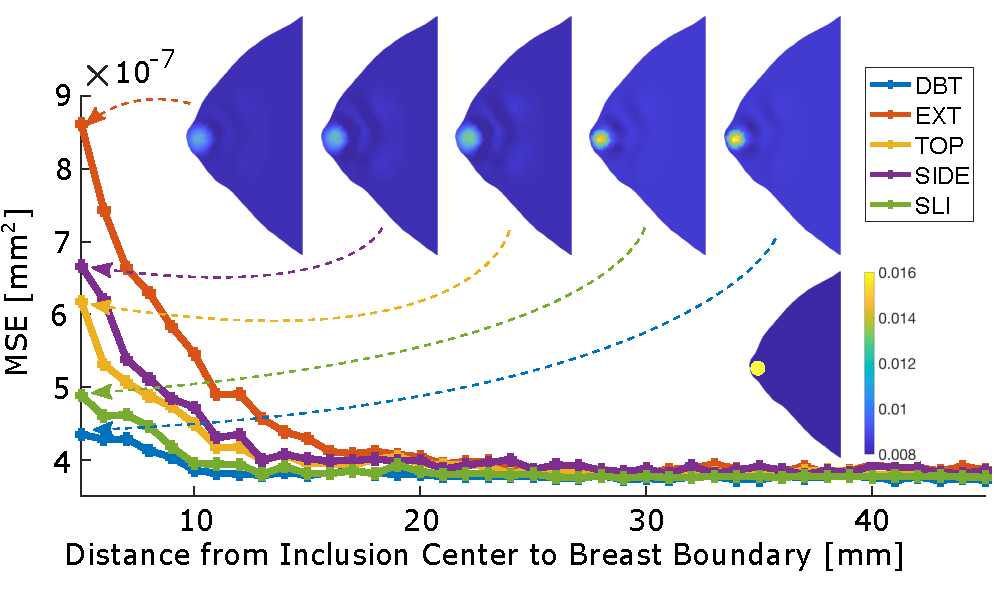
\includegraphics[width=.9\textwidth]{fig/omci/mse.pdf}
	\end{center}
	\caption{A comparison between the mean squared error (\ac{MSE}) of the reconstructed absorption map using 4 estimated surfaces (EXT - $z$-axis extrusion, TOP - sweeping $x/y$ contour along $y/z$ contour, SIDE -- sweeping $y/z$ contour along $x/y$ contour, and \ac{SLI} -- surface acquired from our \ac{SLI} system) as well as the ground truth surface (\ac{DBT}). A 1~cm diameter spherical inclusion is moved away from the breast surface at various depths between 5 and 45~mm in 1 mm increments. Image slices (in $x/y$ plane) of the reconstructed absorption coefficient ($\mu_a$ in mm$^{-1}$) (top-row) and the ground truth $\mu_a$ (bottom-right) are shown as insets.}
	\label{fig:mse}
\end{figure} 

\ac{DOT} reconstructions were performed using our in-house data analysis toolbox, Redbird-m~\cite{Redbird2008}. An $L$-curve analysis is used to determine the regularization parameter as $3.16\times 10^{-10}$, which is fixed over 10 Gauss-Newton iterations. The absorption coefficient of the spherical inclusion was set to be twice ($\mu_a=0.016$/mm) that of the background tissue ($\mu_a=0.008$/mm). The reduced scattering coefficient $\mu_s'$ was set to $1$~mm$^{-1}$ for both breast and inclusion tissues. A set of 32 (16 vertical, 16 horizontal) moving-bar source patterns~\cite{Yao2015} covering an area of 40$\times$40~mm$^2$ was centered at the spherical inclusion. Iso2Mesh was used to interpolate nodal values from the reconstructed mesh to the ground truth mesh based on linear interpolation in order for all reconstructed meshes to have the same number of nodes.

The \ac{MSE} errors from these reconstructed images are summarized in Fig.~\ref{fig:mse}, showing the effect of different surface estimation methods on the accuracy of optical property recovery. Overall, surface mesh accuracy appears to have a notable impact on relatively shallow tumors, with a depth of less than 25~mm. \ac{MSE} values obtained using the \ac{SLI} method closely follow those using the ground truth \ac{DBT} mesh for most inclusion depths. The top- and side-sweep-based meshes followed similar trends, however, reporting higher errors compared to \ac{SLI} especially when the tumor is relatively shallow. The maximum \ac{MSE} value for the \ac{SLI} mesh at a distance of 5~mm from the surface ($4.89\times 10^{-7}$~mm$^2$) was 23\% higher than the maximum \ac{MSE} value for the \ac{DBT} mesh ($4.35\times 10^{-7}$~mm$^2$). In contrast, the single-axis-extrusion method (EXT) \ac{MSE} was nearly twice higher ($8.62\times 10^{-7}$ mm$^2$) than that from the \ac{DBT} mesh. Although the \ac{DBT} and \ac{SLI} mesh \ac{MSE}s plateau to their minimum around 15~mm from the surface, top-, side-, and extrusion-based mesh \ac{MSE}s continue to decrease until a depth of 25~mm. Beyond the depth of 25 mm, the errors between different methods become minimal.

\subsection{Full system \textit{in-vivo} patient results}
\begin{figure}[]
    \begin{center}
    \subfigure[]{\label{fig:PatientResultsA}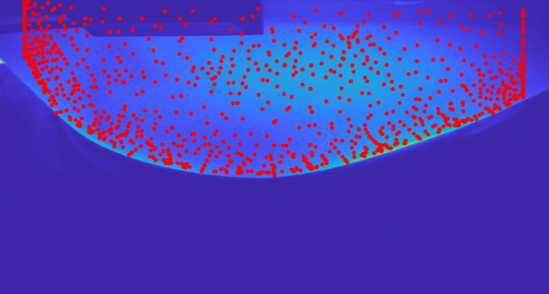
\includegraphics[width=.4\textwidth]{fig/omci/SLIMeshC.png}}
    \subfigure[]{\label{fig:PatientResultsB}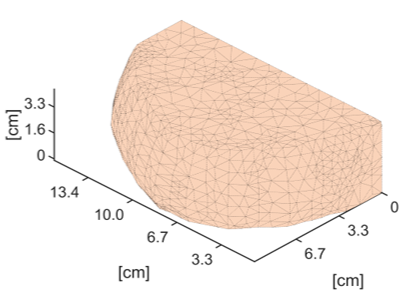
\includegraphics[width=.4\textwidth]{fig/omci/SLIMeshD.png}}
    \subfigure[]{\label{fig:PatientResultsC}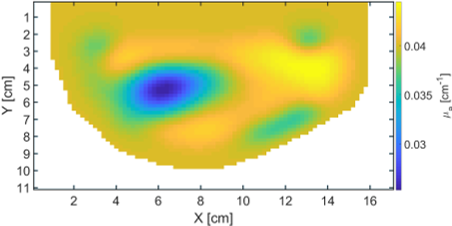
\includegraphics[width=.4\textwidth]{fig/omci/PatientResultsA.png}}
    \subfigure[]{\label{fig:PatientResultsD}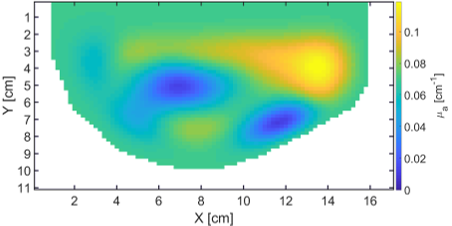
\includegraphics[width=.4\textwidth]{fig/omci/PatientResultsB.png}}
    \end{center}
    \caption{\textcolor{red}{These images will be replaced with patient data showing SLI in a healthy volunteer. I will also show reconstructed results and will cite Edward + Miguel. Edward to provide me with patient IDs that have good SLI acquisitions. } (b) The generated 3D breast-shaped mesh from a \ac{SLI} measurement on a healthy patient.} 
    \label{fig:PatientResults}
\end{figure} 

%Danvers, IRB approved, healthy subject, prior x-ray within X months.
%Acquisition time, time in compression for each breast. 
%Make sure patient we choose has a nipple (so we can see the \ac{SLI} recovery). 
%Find a patient with registered data. 



\section{Discussion}
\label{chap:omci:discussion}

% SLI results - reprojection errors
The camera and projector re-projection errors in Section~\ref{ssec:calibrationresults} represent an average error of fewer than 0.5 pixels in estimating the corner locations of a calibration checkerboard placed between 50 and 250~mm away [Fig.~\ref{fig:mammography_side}] from the projector for all 35 checkerboard positions. Although the same illumination patterns and calibration checkerboard positions were used to calibrate each camera-projector pair, we find a slightly better calibration accuracy when the projector is paired with Camera 1 since Camera 1 is closer to the projector's lens (Fig.~\ref{fig:mammographysetup}). The discrepancy in the re-projection errors of the two pairs is due in part to the asymmetry of the dual-camera setup. The asymmetry arises from the projector offset relative to its housing, making one camera closer to the projector than the other [Fig.~\ref{fig:mammography_top}]. 

% SLI results - surface errors
From Table~\ref{tab:residuals}, the single-axis extrusion method resulted in the highest surface error because it does not account for the curvature of the breast in the $y/z$ plane [Fig.~\ref{fig:mesh_extrude}]. Table~\ref{tab:residuals} indicates that, on average, points in the extrusion-method-derived surface estimation mesh are approximately 6.84~mm away from the \ac{DBT} mesh. The top- and side-sweep methods decrease the surface estimation error by incorporating a second breast contour from the $y/z$ plane [Figs.~\ref{fig:mesh_topsweep} and \ref{fig:mesh_sidesweep}]. Both methods improve the accuracy of surface estimations by approximating the 3-D curvature of the breast. We want to point out that both top-sweep and side-sweep methods require an additional camera to obtain two orthogonal views of the breast~\cite{Pinto2020}, which does not necessarily lead to simplified hardware compared to the \ac{SLI} setup considering the mounting space constraints and lighting conditions~\cite{Rodriguez2017}. While also requiring two cameras, our mammography-tailored \ac{SLI} system can produce sub-millimeter resolution of the surface compared to the reference \ac{DBT} breast model based on Table~\ref{tab:residuals}.

% SLI results - MSE
Our results also demonstrated that the improvement in surface estimation accuracy can lead to improved \ac{DOT} reconstruction accuracy. Fig.~\ref{fig:mse} shows using breast surfaces derived from \ac{SLI} can accurately recover the absorption profile compared to those recovered using the ground-truth (\ac{DBT}) mesh at most tested tumor depths. For superficial/shallow ($<$ 10~mm) tumors, the top- and side-sweep surface estimation methods followed similar trends to each other, reporting \ac{MSE}s about 50\% higher compared to those from using ground-truth (\ac{DBT}) surface models, and about 30\% higher than those from using \ac{SLI} surfaces. As expected, the effect of the surface accuracy decreases as the inclusion is moving further away ($>$ 25~mm) from the skin.

% Patient results - to be added after patient results are added
%In patient measurements, the \ac{SLI} subsystem successfully adjusted its projector intensity to prevent webcam saturation. The recovered bulk breast tissue optical properties from the \ac{FD} subsystem followed the reported values from our group~\cite{Fang2009} and others~\cite{Durduran2002}. Moreover, the 3-D reconstruction of the tissue physiology parameters resembles the internal breast tissue structures (i.e. adipose, muscle, and fibroglandular tissue) described previously~\cite{Fang2009}, denoting the capability of our system to resolve breast compounds.

%limitations
Despite the ability to produce sub-millimeter resolution of breast surfaces in poorly lit and confined mammography-like settings, both our \ac{SLI} system and our analysis have limitations. Firstly, the span of the output point-cloud from our \ac{SLI} system is limited to the area of the breast that is well-illuminated by the projector. As a result, tissue boundaries near the chest wall or those in direct contact with the compression plate may not be well covered due to the limited angles of the projector/camera line-of-sight. Still, for \ac{DOT} of a compressed breast, capturing a significant portion of the front-facing breast tissue as our system does, provides quantitative differences in reconstructions, as shown above. Future improvement of this system should consider using more compact, wide-angle projectors, higher resolution cameras, and patterns with higher order binary codes to both expand the field-of-view and increase the point-cloud resolution. Secondly, a 3-D printed breast model was used to experimentally compare different shape acquisition methods. Different choices of extruder sizes, filament colors, and printing techniques could impact the surface texture of the printed phantom and slightly alter the surface estimation errors. Finally, the quantification of reconstruction errors was based on simulations using a single set of pre-determined breast models, tumor size and shape, tumor contrast, and wide-field pattern size. An experimental validation using heterogeneous phantoms may produce more realistic comparisons.

% CONCLUSION GOES INTO THE CONLUSION OF THE ENTIRE THESIS

% --- EOF ---
% 3dprint.tex:

\chapter{3-D PRINTED PHANTOMS} % all caps please
\label{chap:3dprint}

\section{Introduction}
In order to evaluate the performance of the \ac{NIR} systems we have built, we need to use phantoms. Phantoms are physical samples carefully made to mimic the optical properties of human tissues\cite{Pogue2006}. By imaging these objects of known optical properties, we can evaluate the accuracy of a new system by comparing its result against existing systems. Creating these phantoms is complex: not only do you need to create recipes that lead to desired optical properties, but phantoms must also be manufactured in specific geometries tailored to what the \ac{NIR} system will measure. To address the optical properties, phantom makers tend to focus on mimicking the absorption coefficient ($\mu_a$) and the reduced scattering coefficient ($\mu_s^{'}$) of biological tissue~\cite{Dempsey2017} by using mixtures of scattering agents and absorbing pigments with a clear base~\cite{Hebden1995, Dong2015}. The shape of the phantom is typically created using traditional fabrication techniques, either mold casting~\cite{Hahn2012} or spin coating~\cite{Park2013}. 

Traditionally, as \ac{NIR} imaging was in its infancy, these methods sufficed for simple phantoms. However, these methods fall short of supporting complex geometries. As new \ac{NIR} systems are developed to image the brain~\cite{Hebden2002, Villringer1997} and the breast, we will need to evaluate their performance with phantoms that have complex structural and physiological properties. While some phantom makers use intricate methods and procedures to develop geometrically complex phantoms~\cite{Mobashsher2014}, these phantoms take days to manufacture, require lots of equipment and expertise, and the manual process leads to  geometry and optical property variations due to human variability. Thus, to support the system development, calibration, and testing of new imaging methods~\cite{Cerussi2012, Diep2015} (like the \ac{NIR} systems developed in this thesis), we need a new method to manufacture phantoms with spatially varying optical properties and anatomically accurate geometries.

Rather than add structure-generating methods to traditional phantom making, we propose a method to add customizable optical properties to a digital fabrication method that is already engineered to produce arbitrary geometry---\ac{FDM}. \ac{FDM} is a form of 3-D printing that creates a 3-D object by adding solid material layer-by-layer~\cite{Dong2015}. While traditional 3-D printing uses a single filament material to generate a 3-D object, we proposed the mixing of grey (absorbing), white (scattering), and transparent (base) filament colors to produce the desired optical properties. 

3-D printing for phantom development allows for customizable properties using raw printing materials and the creation of spatially varying optical properties within a 3-D printed phantom. This allows the creation of a wide range of phantoms with precisely known optical properties, geometries, and inclusions of various resolutions (size, shape, depth). Most significantly, the design of a 3-D printed standardized calibration phantom for DOT minimizes geometry and optical property variations due to human variability. In this way, researchers can manufacture identical phantoms using \textit{in-situ} materials with resolutions limited only by their 3-D printer, effectively allowing independent DOT systems to be characterized by the same exact phantom. 

In this chapter, we will detail our method to develop 3-D printed phantoms. We will first describe a workflow to characterize new filaments to account for variations in lots of the same color filament. We then show details of a slicer with the ability to slice an assembly of multiple STL files. The slicer is able to assign filament ratios (tissue types) to each individual STL, allowing the printer to adjust the mixing ratio of the extruder as it prints embedded inclusions into the large geometric print. To demonstrate the capabilities of the slicer, we will slice anatomical geometries with multi-tissue types for each of the three \ac{NIR} systems in this study, including a finger with arteries for \ac{MOXI}, a head phantom with spherical inclusions for use with \ac{MOBI}, and a breast-shaped phantom with inclusions for \ac{OMCI}. Finally, in order to encourage the use of our method, we will disclose a list of lessons learned to help others attempt to replicate our phantoms. 



\section{3-D Printing Hardware}
This project utilizes an experimental \ac{FDM} multi-material 3-D printer (QuadFusion, M3D). This marlin-based printer has an extrusion bar-based frame and uses stepper motors to control motion. The extrusion head is composed of small stepper motors to guide four filaments through a metal nozzle with a \ac{PTFE} insert. The \ac{PTFE} insert is a cylindrical piece with 4 milled holes that extend from end to end. Mixing occurs in the nozzle tip. Due to the need to mix filaments into one nozzle exit, we used \ac{PETG} instead of the standard \ac{PLA} filament. \ac{PLA} is the most popular thermoplastic for 3-D printing because of its cost, ease of print (it is semi-flexible and very forgiving), and it does not off-gas any fumes. However, \ac{PLA} is difficult to mix with other materials due to its limited temperature range. At high temperatures (above 200\textdegree~Celsius), \ac{PLA} releases water which causes a high-pressure build-up in nozzles. To resist the higher temperate and water, \ac{PETG} is used. \ac{PETG} is more viscous at higher temperatures, allowing it to easily fuse with other \ac{PETG} filaments. 


\section{New Filament Characterization}
The filament profiles are the derived settings used for a particular filament. Although the majority of printing settings are consistent across \ac{PETG} filaments, certain features must be accounted for, particularly, the extrusion multipliers and retraction amount. \ac{EM} is a setting used to account for variability in extrusion amounts. An extrusion multiplier of 1 means that 1~mm of filament is extruded for every 1~mm requested. Due to the filament path (the Bowden tube, motor teeth, varying temperatures), certain filaments in certain printers may require over- or under-extrusion to extrude the correct amount of filament. The retraction amount is the amount of filament to pull back up into the nozzle as the print head moves in between printing layers. When this value is too low, you will see ``stringing'' in prints from the oozing of material while the head is in motion. Too much retraction and the printer will not print the first few millimeters upon restarting since the nozzle is empty of filament.

To account for variations in filaments of the same color by the same manufacturer, we have developed a method to characterize filaments and create filament profiles for each spool of filament. In fairness, the variability in the extrusion multiplier is not entirely due to the manufacturer. The QuadFusion head is a complex head that requires filaments to be driven through curved paths and high pressure that result in friction. We calculate filament-specific \ac{EM}s for each spool used in our printer by printing a square wall with the thickness of a single \ac{PW}. We then calculate the new \ac{EM} based on the desired path width and the actual path width of the print using the formula $EM_{new} = EM_{printed} \times (PW_{desired}/PW_{measured})$. The steps are outlined in Figure~\ref{fig:emflowchart}.

\begin{figure}
	\begin{center}
        \subfigure[]  {\label{fig:emflowchart}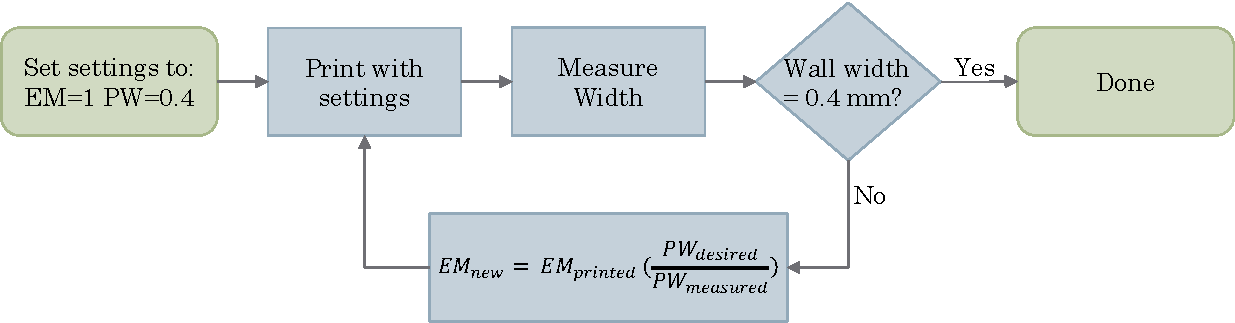
\includegraphics[width=\textwidth]{fig/3dprint/emflowchart.pdf}}
        \subfigure[]{\label{fig:clear}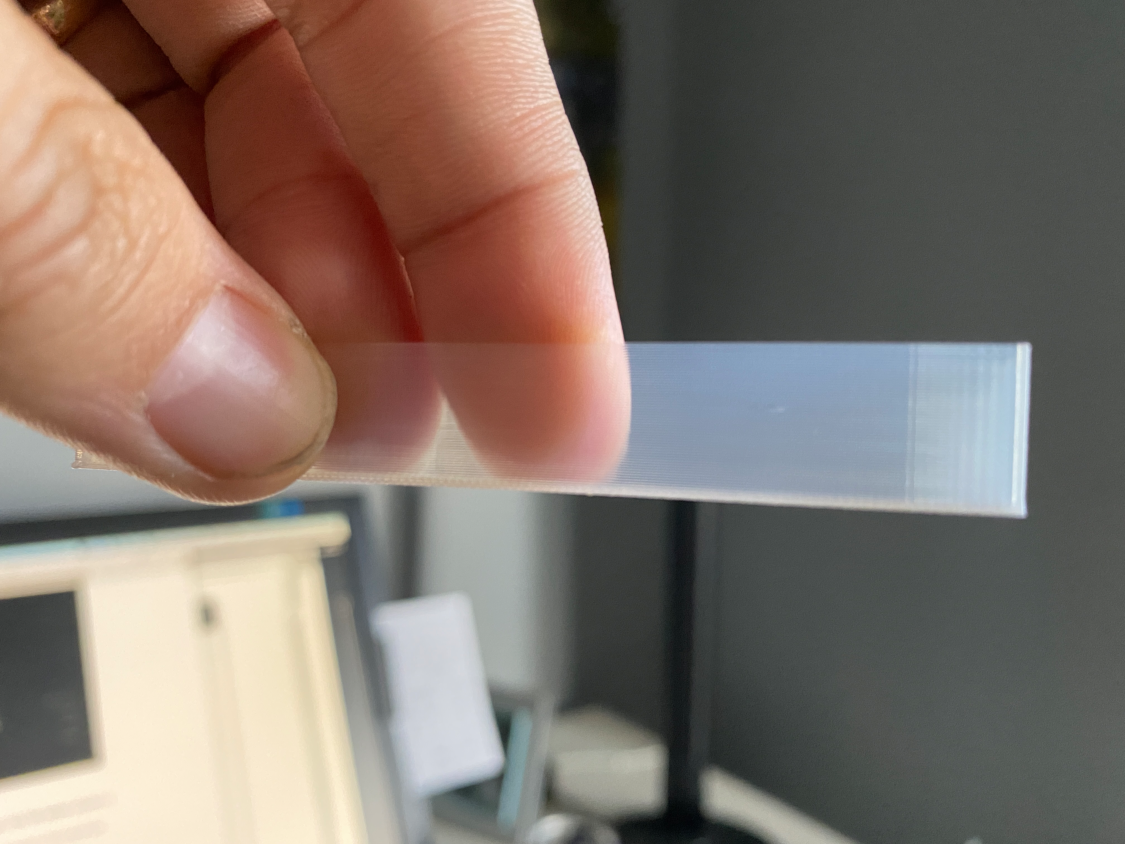
\includegraphics[height=5cm]{fig/3dprint/clear.pdf}}
        \subfigure[]{\label{fig:caliper}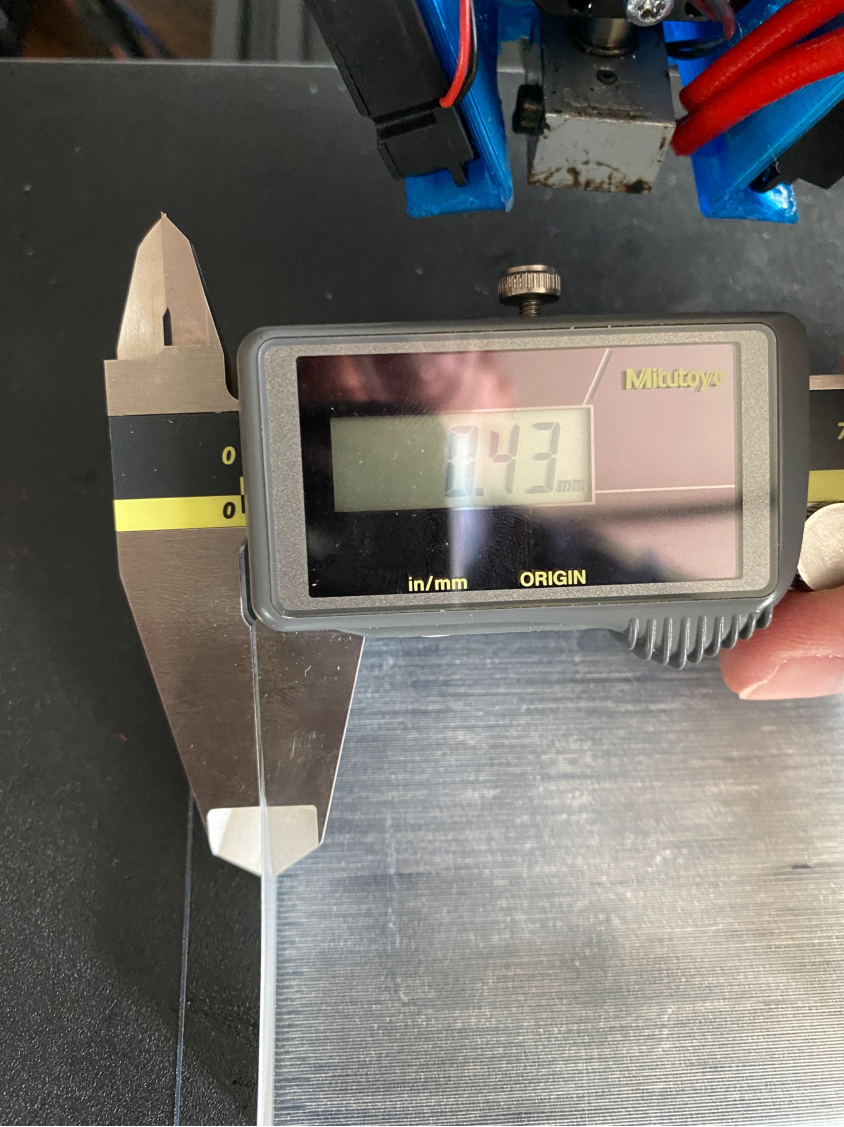
\includegraphics[height=5cm]{fig/3dprint/caliper.pdf}}
	\end{center}
	\caption{(a) Flowchart showing how to use measured path widths to adjust extrusion multiplier values when characterizing filaments. (b) Printed square wall using clear \ac{PETG} filament. (c) Caliper measurements show over-extrusion.} 
	\label{fig:em}
\end{figure} 

A 3-D printed tissue type is simply a mixing ratio of multiple characterized filament profiles. While one filament profile informs of the settings for printing a single filament, we have to create combined printing settings when mixing multiple filaments (tissue types). This is done as a weighted average of the settings scaled by the mixing ratios. For example, if white, grey, black, and clear filaments each have extrusion multipliers of 1, 0.98, 1, and 0.9, respectively, and we want to mix them in a 30/20/0/50 ratio, then the final extrusion multiplier would be
$(1\times30 + 0.98\times20 + 1\times0 + 0.9\times50) / (30+20+0+50) = 0.946$. Similarly, the extrusion motors are driven at scaled rates based on the filament mixing ratio.



\section{Multi-filament slicing}
\subsection{Artifacts for purging during transition}
One difficulty in fused multi-material 3-D printing not found in single filament printing is the need to purge the nozzle in between changing mixing ratios for different tissue types on the same layer. For example, if we want two separate mixing ratios for concentric rods, the nozzle needs to be purged in between printing the outside color and printing the inside color. Purging refers to the extrusion of sacrificial filament when the outputted mixed filament is transitioning between different two ratios (tissue types).

We have implemented a ``caging'' method in which a cage is built around the print to purge the nozzle. The method is an extension of the ``brim'' artifact commonly used to help prints adhere to the print bed. Essentially, at every layer, concentric shapes around the model are printed for each ratio. This allows the nozzle to fully transition to a new mixing ratio prior to continuing the print. This results in a cage around the print. 

\begin{figure}
	\begin{center}
	\subfigure[]{\label{fig:caging01}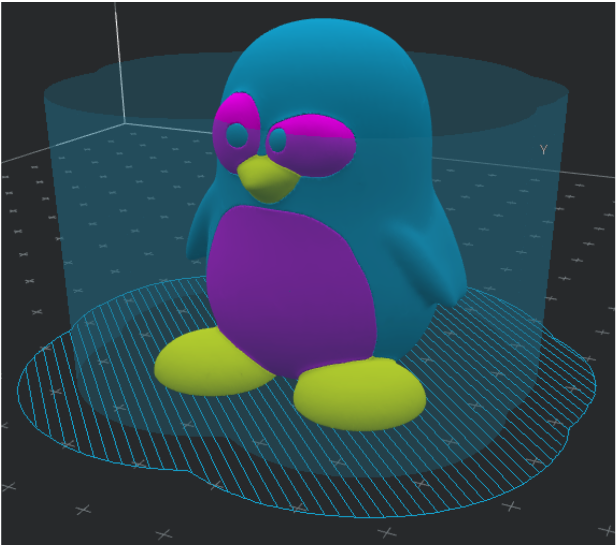
\includegraphics[height=4cm]{fig/3dprint/caging01.png}}
	\subfigure[]{\label{fig:caging02}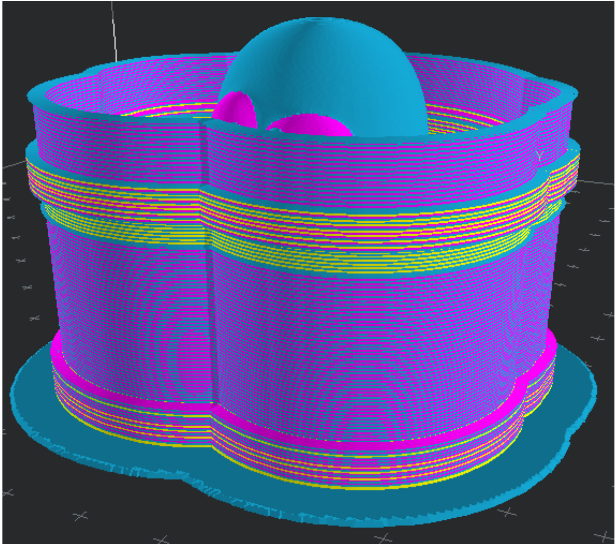
\includegraphics[height=4cm]{fig/3dprint/caging02.png}}
	\subfigure[]{\label{fig:caging03}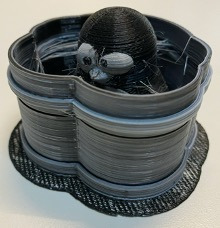
\includegraphics[height=4cm]{fig/3dprint/caging03.jpg}}
	\end{center}
	\caption{The ``caging'' purge method (a) An example penguin composed of three different tissue types. (b) The same penguin model with the cage shown. The colors of the cage indicate the colors on that segment of the print. (c) Resulting 3-D printed penguin. } 
	\label{fig:caging}
\end{figure} 

\subsection{MOXI, MOBI, and OMCI system slicing} % cannot use \ac{} in section titles



\section{Lessons learned for use of PETG in filament mixing} % cannot use \ac{} in section titles
The use of \ac{PETG} filament, a ``caging'' purging method, mixed filament ratio-based extrusion multipliers, and an experimental \ac{FDM} 3-D printer has taught us many lessons. To facilitate future researchers in this space, here is a list of lessons learned and pitfalls to avoid. 

\begin{itemize}
    \item BED MATERIAL: \ac{PETG} sticks very well to the printing bed. The use of sacrificial generic blue painter's tape on the print bed will facilitate removal by removing the print from the bed by pulling on the tape itself.
    \item BED LEVELING: Add a decent gap between the nozzle and the bed. Typical 3-D printers level the bed by using a single sheet of regular printing paper as the unit of measure between the nozzle and the print bed. To account for the ``gooey''-ness of \ac{PETG}, use 3 sheets of paper.
    \item BED TEMPERATURE: Start the bed temperature around 80\textdegree~C. Do not heat above 100\textdegree~C. Higher bed temperatures are better for bed adhesion, but \ac{PETG} already adheres pretty well. Consider decreasing the space between the nozzle and the bed before increasing the bed temperature. 
    \item NOZZLE TEMPERATURE: \ac{PETG} prints between 230 and 250\textdegree~C. However, \ac{PTFE} (which is what the tube that aligns the filaments prior to being mixed in the nozzle is made of) has a melting point between 250 and 260\textdegree~C. Start at 230\textdegree~C and do some test prints. If you hear a knocking noise during printing, your extruder is skipping, and you should increase the nozzle temperature by 5\textdegree~C. 
    \item RETRACTION SPEEDS: Do not retract \ac{PETG} at high speeds. Set the retraction speed to around 25~mm/s. The retraction distance should be set at about 3 or 4 millimeters for direct drive extruders. With \ac{PETG}, the retraction speed is more important than distance. If you still have oozing and stringing, try lowering the retraction speed.
    \item TRAVEL SPEED: One more parameter that will help in reducing oozing is the travel speed. \ac{PETG} tends to drip from the tip of the nozzle, especially if the nozzle temperature is high. To combat this, try increasing the travel speed to reduce the time the printer is not actively extruding.
    \item PRINT SPEED: \ac{PETG} is very sensitive to print speed. Printing too fast results in poor layer adhesion, extruder skipping, and low print quality. Printing too slow results in deformed parts, stringing, and oozing. A good place to start is between 50 and 55~mm/s. We suggest 25~mm/s for the first layer and the outer wall, while travel moves should be as fast as possible, at least 120~mm/s, to avoid oozing.
    \item FANS: We recommend printing without fans for the first two layers. All other layers should have the fan running at 100\%. 
\end{itemize}


% --- EOF ---
\chapter{CONCLUSION} % all caps please
\label{chap:conclusion}

In this thesis we ....

\section{Pugh Chart}

Finally, we revisit the system lifecycle properties defined in Table~\ref{tab:ilities}. We use the Pugh method~\cite{Pugh1981} to qualitatively rank each of the three \ac{NIR} systems against a reference design using the ilities as the set of criteria. The reference \ac{NIR} system is a standard finger-clip-based, two-wavelength pulse oximeter. Each ility can vary between $\pm3$ indicating that the system is ranked better ($+$), worse ($-$), or the same as ($0$) the reference design. A value of 3 allows for each of the three systems to all be ranked better (or worse) than the reference design while still providing relative ranking between the three systems. The results of this ranking are shown in Table~\ref{tab:pughtable}. 

\begin{table}[]
\centering
\caption{Pugh Chart ranking of \ac{NIR} systems}
\label{tab:pughtable}
%\resizebox{\textwidth}{!}{%
\begin{tabular}{@{}lcccc@{}}
\toprule
Ility Name        & Pulse Oximeter & MOXI & MOBI & OMCI \\ \midrule
Adaptability      & 0              & 0    & 3    & 1    \\
Affordability     & 0              & 2    & -1   & -3   \\
Comfortability    & 0              & -1   & 3    & -3   \\
Conformability    & 0              & -1   & 3    & -1   \\
Extensibility     & 0              & 2    & 1    & 3    \\
Interoperability  & 0              & 0    & 3    & 2    \\
Maintainability   & 0              & 3    & -1   & -3   \\
Manufacturability & 0              & 3    & -1   & -3   \\
Modifiability     & 0              & 1    & 2    & 3    \\
Operability       & 0              & -1   & -2   & -3   \\
Portability       & 0              & 3    & -1   & -3   \\
Reconfigurability & 0              & 1    & 2    & 0    \\ \bottomrule
\end{tabular}%
%}
\end{table}

\begin{description}
   \item[Adaptability] \ac{MOXI} is designed for a specific function and is not easily adaptable for other vital signs. \ac{OMCI} can be adapted for other applications. For example, the \ac{SLI} system can be used on its own for surface estimation of other body parts (e.g. facial landmark identification). It is \ac{MOBI}, however, that is ranked highest dues to its modular design that allow for spectroscopy or \ac{DOT} applications at various sites. 
   
   \item[Affordability] \ac{OMCI} is clearly the most expensive \ac{NIR} system we built due to its numerous subsystems and expensive hardware. Although \ac{MOBI} has similar optical components as a traditional pulse, it does use more complex electronics and interfaces that drive up the cost. In contrast, the \ac{MOXI} is more affordable that traditional pulse oximeters since it only requires a small piece of paper. The reason for give it a rank of three is because \ac{MOXI} still requires a smartphone, which a user may or may not have in their possession. 
  
   \item[Comfortability] The silicone covers and wireless capability of the \ac{MOBI} modules allow them to be used for hours at a time. On the other hand, \ac{OMCI} requires heavy compression of the breast to minimize the thickness between paddles. This is so uncomfortable that we have to limit the time in compression to less than 3 minutes. The \ac{MOXI} system, although highly portable, requires the user to actively press onto the camera phone, which can cause discomfort over long-term use compared to the passive design of a traditional finger-clip pulse oximeter. 
   
   \item[Conformability] The reflectance-based design of \ac{MOXI} relies on the flat surface of a phone camera that is susceptible to motion. \ac{OMCI}, like \ac{MOXI}, uses flat surfaces that compress the breast preventing motion. However, the mechanical principle of compressing tissue using two fixed-shaped surfaces is identical to a traditional pulse oximeter in the sense that neither adjusts to different user shapes. In contrast, the flexible-circuit-based \ac{MOBI} modules conform easily to the scalp. 
   
   \item[Extensibility] Given the context, our \ac{OMCI} system be easily extended to include features from state-of-the-art \ac{DOT} research including the use of optimal wide-field illumination patterns and sizes, new \ac{SLI} illumination patterns, and compression-sensor-based tomography.  In contrast, \ac{MOBI} would leverage features from portable fNIRS systems, which rely on the use of new driving electronics and optodes, which require new circuit designs. It, however, unlike a pulse oximeter, vary the intensity of light to accomodate hair artifacts. \ac{MOXI} can do software update easily, but features to support other vital signs necesitate specific electronics that the mobile-phone in use may not have. 
   
   \item[Interoperability] \ac{MOXI} is not better or worse in its ability to operate with other imaging systems. By design, \ac{OMCI} is capable of being integrated in existing x-ray mammography systems. However, \ac{MOBI} receives the highest score due to the auxiliary input of the master module, allow its measurements to synchronize with any other system that can output a \ac{TTL} signal. 
   
   \item[Maintainability] Our \ac{MOXI} system is ranked highest because it can be easily maintained with regular software updates and replacing its inexpensive pieces of paper. Our \ac{MOBI} modules are robust and designed to be used in natural settions. However, they were ranked lower than the reference design due to the high number of components (flat-flex cables, caps, master modules) that can potentially break and require replacement. Due to the complexity of our \ac{OMCI} system, it is ranked the lowest in maintainability.
   
   \item[Manufacturability] \ac{MOBI} modules have very similar optical components to a finger-clip pulse oximeter, thus same expertise used in designing the circuit and fabricating the physical enclosure of a pulse oximeter clip is needed for fabricating a \ac{MOBI} module. We ranked them $-1$ because a \ac{MOBI} system also requires the fabrication of the master and trigger boards, as well as the creating of the headgear that holds the modules in place. Our \ac{OMCI} system requires not only fabricating circuits but also mechanical assemblies and sensitive optical fibers. In contrast, \ac{MOXI} simply requires a piece of colored paper. 
   
   \item[Modifiability] Modifiability refers to the ability to change a default set of specified parameters. Besides the color of the paper filter, \ac{MOXI} does not allow any user changes. On our \ac{MOBI} system, a use can change the source currents, detector gains, and sampling strategy (sequentialy and spatial multiplexing). \ac{OMCI} receives the highest ranking in this category due to the ability to change the wide-field and \ac{SLI} patterns, position of the \ac{RF} source location, and scaling factor sensitivity. 
   
   \item[Operability] Although a lot of consideration was taken into the usability of the software \ac{GUI} of our \ac{OMCI} system, it is clear from the extensive training that was required to obtain human subject data that the complexity of all the subsystems and calibration steps prior to acquisition make this system difficult to use, even for a knowledgeable user. Although conceptually similar to a pulse oximeter, our \ac{MOBI} modules require relatively longer setup times to connect modules and affix a cap onto a user. Our \ac{MOXI} system only requires user input into a very basic application. Also easy to operate, it is ranked less than zero because a finger-clip-based pulse oximeter requires no user input.
   
   \item[Portability] Our \ac{MOXI} system receives the highest ranking because it only requires a piece of paper and its Moximeter application can be easily downloaded. Although wearable and portable, compared to a traditional pulse oximeter, our \ac{MOBI} system requires the transportation of multiple modules and supporting electronics. Our \ac{OMCI} breast imaging system is much less portable than a pulse oximeter due to its size and weight.
   
   \item[Reconfigurability] \ac{OMCI} requires a well-aligned and calibrated system to function. In theory, \ac{MOXI} can use different colored paper filters and the Moximeter application attempts to account for the misplacement of the filter on the camera. \ac{MOBI} is by far the most reconfigurable of the three \ac{NIR} systems by simply reconnected the modules in different arrangements. However, the optode layout within a \ac{MOBI} module is fixed, which is why the rank is set to two. 
\end{description}



% --- Bibliography ----
\bibliographystyle{unsrt} % in order of appearance, not alphabetical

% include bibliography definition
\bibliography{bib/thesis}


% --- Appendix ---
%\appendix
%include anything you need in the appendix
%\include{appendix/appendix}


% --- Index ----
%\printindex


% --- that's it ---
\end{document}

% --- EOF --------------------------------------------------------------------

